\documentclass[a4paper,11pt]{article}
\pdfoutput=1 % if your are submitting a pdflatex (i.e. if you have
             % images in pdf, png or jpg format)

\usepackage{jcappub} % for details on the use of the package, please
                     % see the JCAP-author-manual

\usepackage[T1]{fontenc} % if needed
\newcommand{\ek}[1]{\textcolor{blue}{[{\bf EK}: #1]}}
\allowdisplaybreaks

\title{\boldmath Halo formation through aspherical collapse in ultra-light dark matter}





%% %simple case: 2 authors, same institution
%% \author{A. Uthor}
%% \author{and A. Nother Author}
%% \affiliation{Institution,\\Address, Country}

% more complex case: 4 authors, 3 institutions, 2 footnotes
\author[a]{Emily Kendall}
% \author[c]{S. Econd,}
% \author[a,2]{T. Hird\note{Also at Some University.}}
% \author[a,2]{and Fourth}

% The "\note" macro will give a warning: "Ignoring empty anchor..."
% you can safely ignore it.

\affiliation[a]{The University of Auckland, Private Bag 92019\\
Auckland 1142, New Zealand}
% \affiliation[b]{Another University,\\different-address, Country}
% \affiliation[c]{A School for Advanced Studies,\\some-location, Country}

% e-mail addresses: one for each author, in the same order as the authors
\emailAdd{eken000@aucklanduni.ac.nz}
% \emailAdd{second@asas.edu}
% \emailAdd{third@one.univ}
% \emailAdd{fourth@one.univ}




\abstract{Ultra-Light Dark Matter [ULDM] offers an interesting alternative to the $\Lambda$CDM paradigm, popular in part because of its perceived potential to resolve the contentious `small-scale crisis' of CDM. While the predictions of ULDM and $\Lambda$CDM converge on cosmological scales, it is necessary to understand the precise differences between the predictions of these models on small (kiloparsec) scales. A unique feature of ULDM on these scales is the presence of wave-like interference effects in the underlying dark mater density distribution. One consequence of these wave effects is gravitational cooling, a process by which overdensities can loose mass by ejection of the scalar field through scattering of interference fringes. In this work, we examine the consequences of gravitational cooling on the collapse of ellipsoidal overdensities, contrasting this behaviour with the Zel'dovich type triaxial collapse associated with CDM. We consider how this process varies with ULDM particle mass and ellipticity or flattening of ellipsoidal overdensities. Because the presence of propagating wavefronts means that a collapsing overdensity distribution in ULDM contains extended anisotropic structures, we also examine the statistics of the eigenvalues of the traceless tidal tensor. Unlike the standard 2-point correlator, this allows us to preserve information about anisotropies in the underlying distribution. We remark that such a statistical analysis could prove useful in discriminating between ULDM and CDM models by comparison of the large-scale cosmic web structure, which in the case of ULDM may contain non-trivial interference pattern within filaments.}



\begin{document}
\maketitle
\flushbottom

\section{Introduction}
\label{sec:intro}

    % \item effect of delta rho (ratio of overdensity)
    % \item need to quantify angular momentum section

As direct-detection experiments continue to constrain the viable parameter space of weakly interacting cold dark matter \cite{Schumann:2019eaa}, interest in alternative dark matter models grows. Ultra-Light Dark Matter [ULDM] presents an alternative to $\Lambda$CDM which, while maintaining agreement on cosmological scales, possesses novel features on small (galactic) scales \cite{Hui:2016ltb}. This small-scale disparity is due to the macroscopic de Broglie wavelength associated with the constituent particle's extremely small mass ($\sim10^{-22}$eV). Because of this large de Broglie wavelength, astrophysical processes such as the collapse of overdensities or the collisions of ULDM halos can be expected to induce complex interference effects. Indeed, imprints of interference patterns are expected to be manifest in the filamentary structure of the cosmic web \cite{Mocz:2019emo}. It is therefore of interest to understand the stucture formation process in the ULDM model, beginning with the collapse of overdensities in an expanding background, and examining the impact of macroscopic interference effects. 

In this paper we consider isolated ellipsoidal `top-hat' overdensities, which are allowed to collapse in an expanding background and relax to form ULDM halos possessing the typical solitonic core surrounded by an NFW-like outer halo. Our ULDM simulations are performed using the {\sc PyUltraLight} tool \cite{Edwards:2018ccc}, modified to include expansion.
We consider the effects of ULDM particle mass, ellipticity, and angular momentum on the overdensity collapse process. We also consider the impact that wavefront propagation has on the statistical properties of the evolving density distribution. To do this we employ the traceless tidal tensor as a quantity which naturally preserves information about anisotropic structures \cite{Lee:2009uv}. We analyse the 2-point statistics of the eigenvalues of this tensor in order to distinguish between distributions which contain complex interference patterns and those which do not, as is the case for standard CDM.

While {\sc PyUltraLight} is a useful simulation tool with which to perform a preliminary investigation of this kind, it is limited by fixed spatial resolution. This means that large cosmological volumes cannot be simulated whilst maintaining adequate resolution on the scale of the de Broglie wavelength. However, there are currently a number of efforts to develop advanced ULDM simulation tools, some of which make use of adaptive mesh refinement (AMR) \cite{Mocz:2019emo, Niemeyer:2019aqm, Veltmaat:2019hou}. Such tools will allow cosmological structure formation simulations to be undertaken which incorporate baryonic effects and achieve the necessary resolution to characterise interference effects on the de Broglie scale. We therefore hope that this work serves as a proof-of-principle for in-depth investigations utilising the outputs of more advanced simulation tools. 

The structure of this paper is as follows. In Section \ref{sec:sims}, we discuss the simulations of collapsing overdensities using the {\sc PyUltraLight} tool, and discuss how different ULDM particle masses are implemented. In Section \ref{sec:collapse}, we discuss the effects of varying the ULDM particle mass on the collapse of isolated ellipsoidal overdensities. In Sections \ref{sec:flattening} and \ref{sec:rotation} we consider how changing the shape and angular momentum of the initial overdensity affects this process. We briefly diiscuss evidence for variability in the theoretical ULDM core-halo relation in Section \ref{sec:core-halo}. We then perform a statistical analysis of collapsing density distributions in the ULDM model, making use of the eigenvlaues of the traceless tidal tensor in Section \ref{sec:stats}. Finally, we conclude and discuss prospects for further investigation in Section \ref{sec:conclusion}.


\section{Simulation setup}\label{sec:sims}

In this work we generate a series of test density fields using the {\sc PyUltraLight} simulation tool \cite{Edwards:2018ccc}. We first modify this tool to incorporate expansion, assuming a matter dominated evolution of the scale factor, namely $a\propto t^{2/3}$. We also incorporate a sponge at the boundary such that ejected matter does not re-enter the simulation region due to the periodic boundary conditions. We use {\sc PyUltraLight} to simulate the collapse of isolated ellipsoidal overdensities in an expanding background, using different assumptions for the ULDM particle mass, ellipticity, and angular momentum. For a sufficiently light ULDM particle mass, the effects of the macroscopic de Broglie wavelength can be expected to impede the Zeldovich type collapse characteristic of CDM \cite{Zeldovich:1969sb}. However, as the ULDM particle mass is increased, we approach a regime in which the correspondence between the Schr{\"o}dinger-Poisson equations of ULDM and the Vlasov-Poisson equations dictates that the dark matter behaves similarly to standard CDM \cite{Mocz:2018ium}. Therefore, as the ULDM particle mass increases, we recover the Zeldovich type scenario in which collapse occurs most rapidly along the shortest axis of the ellipsoidal overdensity. 

We work in the native dimensionless code units of {\sc PyUltraLight} given by 
\begin{align}
    \CMcal{L}&=\left(\frac{8\pi\hbar^2}{3 m^2H_0^2\Omega_{m_0}}\right)^{\frac{1}{4}}\approx121\left(\frac{10^{-23}\operatorname{eV}}{m}\right)^{\frac{1}{2}}\operatorname{kpc},\label{eq:length}\\
    \CMcal{T}&=\left(\frac{8\pi}{3 H_0^2\Omega_{m_0}}\right)^{\frac{1}{2}}\approx75.5 \operatorname{Gyr},\label{eq:time}\\
    \CMcal{M}&=\frac{1}{G}\left(\frac{8\pi}{3 H_0^2\Omega_{m_0}}\right)^{-\frac{1}{4}}\left(\frac{\hbar}{m}\right)^{\frac{3}{2}}\approx 7\times 10^7\left(\frac{10^{-23}\operatorname{eV}}{m}\right)^{\frac{3}{2}}\operatorname{M}_{\odot}.\label{eq:mass}
\end{align}

In this work we will consider order of magnitude variations in the ULDM particle mass, as this may prove useful for tightening existing mass constraints \cite{Marsh:2018zyw, Armengaud:2017nkf, Irsic:2017yje}.
Working in these units, we can simulate the effects of an increased ULDM particle mass simply by increasing the side length of the simulation region. For example, if we wanted to maintain the same physical initial conditions but with the ULDM mass increased by an order of magnitude, we would need not convert into physical units, but would instead increase the side length of the simulation region by a factor of $\sqrt{10}$ in the dimensionless code units given above. We need not change the density of any input configuration, as it can be seen from the above expressions that the change in the mass unit is exactly cancelled by the change induced by 3 factors of the length unit. Hence, we find it most convenient to work in dimensionless code units, as this obviates the need for an explicit assumption for the ULDM particle mass. Where valuable, we convert quantities of interest into physical units under different ULDM particle mass assumptions to give a sense of scale.

We simulate the collapse of isolated ellipsoidal overdensities, repeating our simulations for different ULDM mass scales, initial ellipticities and angular momenta. The precise details of the simulation setups are discussed in detail in the following sections. Of course, these initial configurations are highly contrived, and thus cannot be expected to generate physically realistic predictions for large scale cosmological structures. We are presently restricted to these toy models as it is not possible to perform astrophysically realistic structure formation simulations using the {\sc PyUltraLight} tool. This is because simulations of large cosmological volumes necessarily sacrifice spatial resolution, meaning that wave-like effects on the ULDM de Broglie scale are not captured. As it is precisely this wave behaviour which is expected to engender differences in the predictions of ULDM and CDM, such simulations are not useful for our analysis. We note, however, ongoing development of much more sophisticated ULDM simulation tools \cite{Mocz:2019emo, Niemeyer:2019aqm, Veltmaat:2019hou}, from which detailed information about structure formation in the ULDM model can be garnered. This work, therefore, provides a groundwork upon which further investigation can build when better simulation data becomes available.



\section{Collapse and gravitational cooling of ellipsoidal overdensities for varying ULDM particle mass}\label{sec:collapse}

We simulated the collapse of randomly oriented ellipsoidal overdensities in an expanding background where the ellipsoid is defined by

\begin{equation}\label{eq:ellipse}
    \frac{x^2}{a^2}+\frac{y^2}{b^2}+\frac{z^2}{c^2} = R.
\end{equation}

The simulation resolution was $300^3$ and $R$ was chosen to be 100 grid spaces\footnote{R is defined in terms of grid spaces since we may assume a different ULDM particle mass and therefore a different simulation side length in dimensionless code units. In each case, however, the \textit{physical} length corresponding to each grid space remains the same.}. Meanwhile the parameters ${a, b, c}$ were initially set to ${3,3,8/9}$. For the first simulation, the side length was set to $10a(t)$ {\sc PyUltraLight} code units, and the constant density within the ellipsoid was set to 2500 code units. If a ULDM particle mass of $10^{-22}\mathrm{eV}$ is assumed, this corresponds to a simulation side length of $\sim 380a(t) \mathrm{kpc}$, and an ellipsoidal overdensity of mass $\approx 7\times 10^9 \mathrm{M}_{\odot}$. Outside of the ellipsoid, the density is rapidly decreased to zero via a Gaussian smoothing.

The ellipsoidal overdensity is initialised at $z=100$, and left to evolve to $z=1.5$. During this time, the overdensity begins to collapse, first inducing interference fringes throughout the simulation region and finally virialising to form a relaxed halo. In the first simulation the side length is set to 10 code units. In the second simulation this is increased to $\sqrt{10}\times 10$ code units, reflecting an order of magnitude increase in ULDM particle mass. Henceforth, we will distinguish between these two scenarios using the designations `$\mathrm{m}_0$' and `$10 \mathrm{m}_0$', avoiding an explicit choice for the ULDM particle mass. 

Figures \ref{fig:contours_light} and \ref{fig:contours_mid} show the (log) density distributions through the central plane of the simulation region for each of the two scenarios (distance not log-scaled). The left panel of Figure \ref{fig:contours_light} shows extended wavefronts emanating from the overdensity near the onset of collapse (z = 99.5) for the $\mathrm{m}_0$ case, while the left panel of \ref{fig:contours_mid} shows significantly reduced wavefronts at the same redshift for $10 \mathrm{m}_0$. In the latter case, the ellipsoid can be seen to be flattening into a `Zeldovich pancake', while in the former case the interference effects are impeding this process. The centre panels of Figures \ref{fig:contours_light} and \ref{fig:contours_mid} show how the wavefronts have evolved at z = 96.5. As expected, the interference effects are much more pronounced in the $\mathrm{m}_0$ case. The rightmost panels of Figures \ref{fig:contours_light} and \ref{fig:contours_mid} show cross-sections through the relaxed halos at z = 1.5. As expected, the size and density contrast of fluctuations is more pronounced in the incoherent outer halo of the $\mathrm{m}_0$ case.  

In both the left and centre panels, artifacts of the cubic simulation grid can be observed as faint straight lines and small square regions of overdensity. These sources of error should be kept in mind when analysing statistical correlations within the simulation. 


\begin{figure}[!htb]
\minipage{0.32\textwidth}
  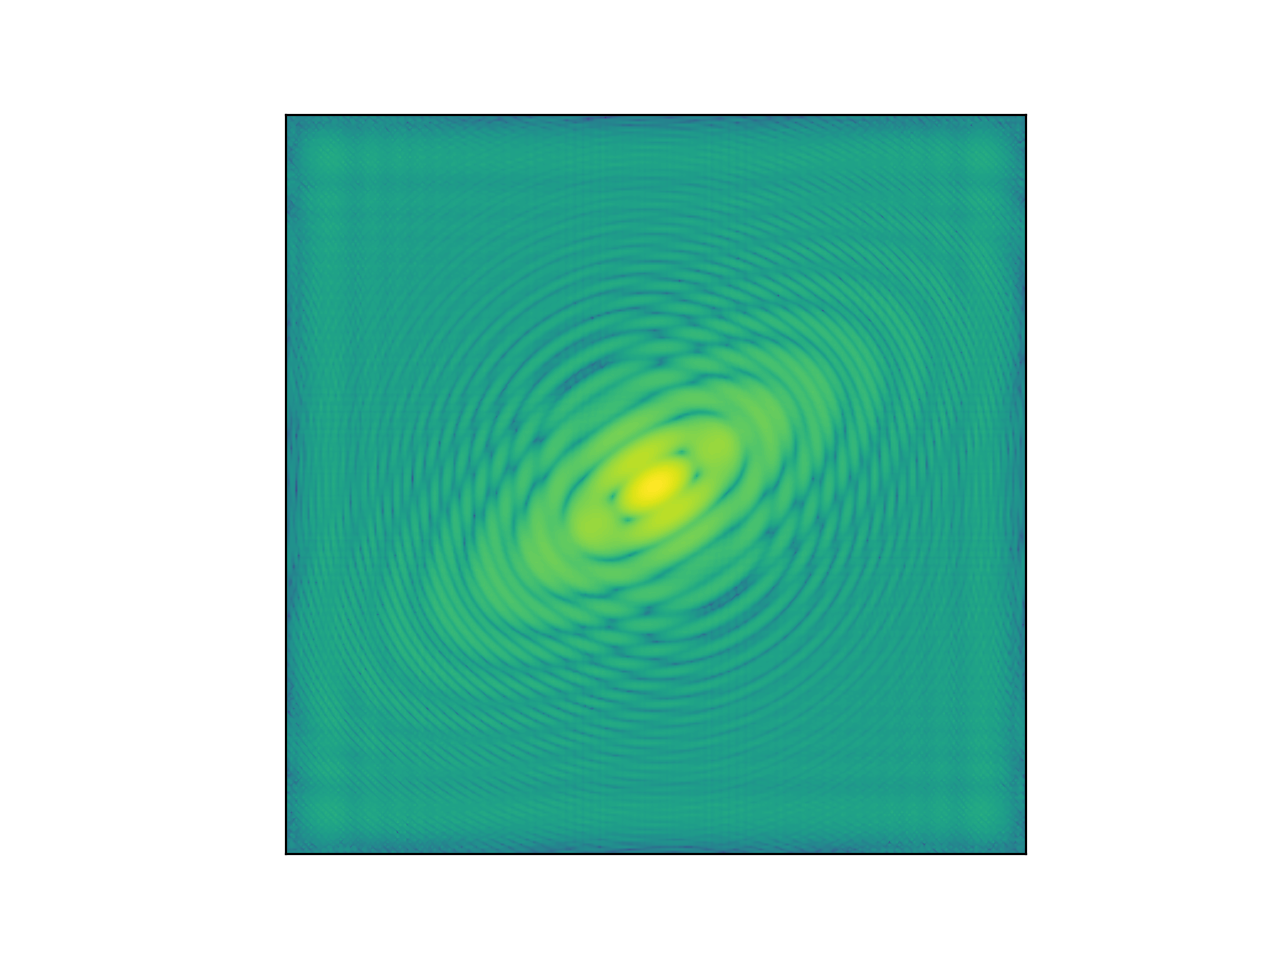
\includegraphics[trim={3cm 0 0 0}, scale=0.5]{single_light_plane_1.png}
\endminipage\hfill
\minipage{0.32\textwidth}
  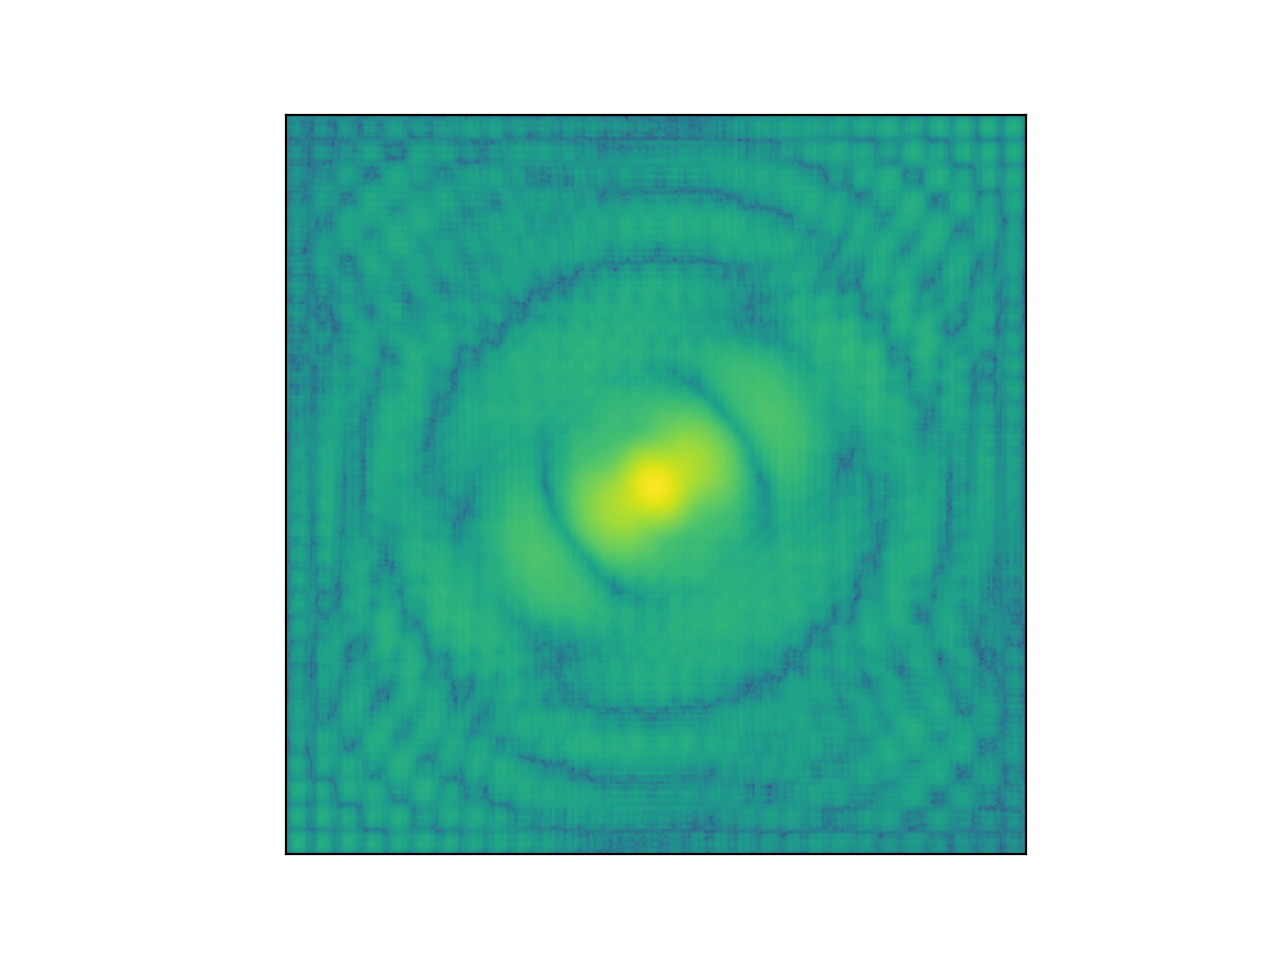
\includegraphics[trim={3cm 0 0 0},scale=0.5]{single_light_plane_7.png}
\endminipage\hfill
\minipage{0.32\textwidth}
  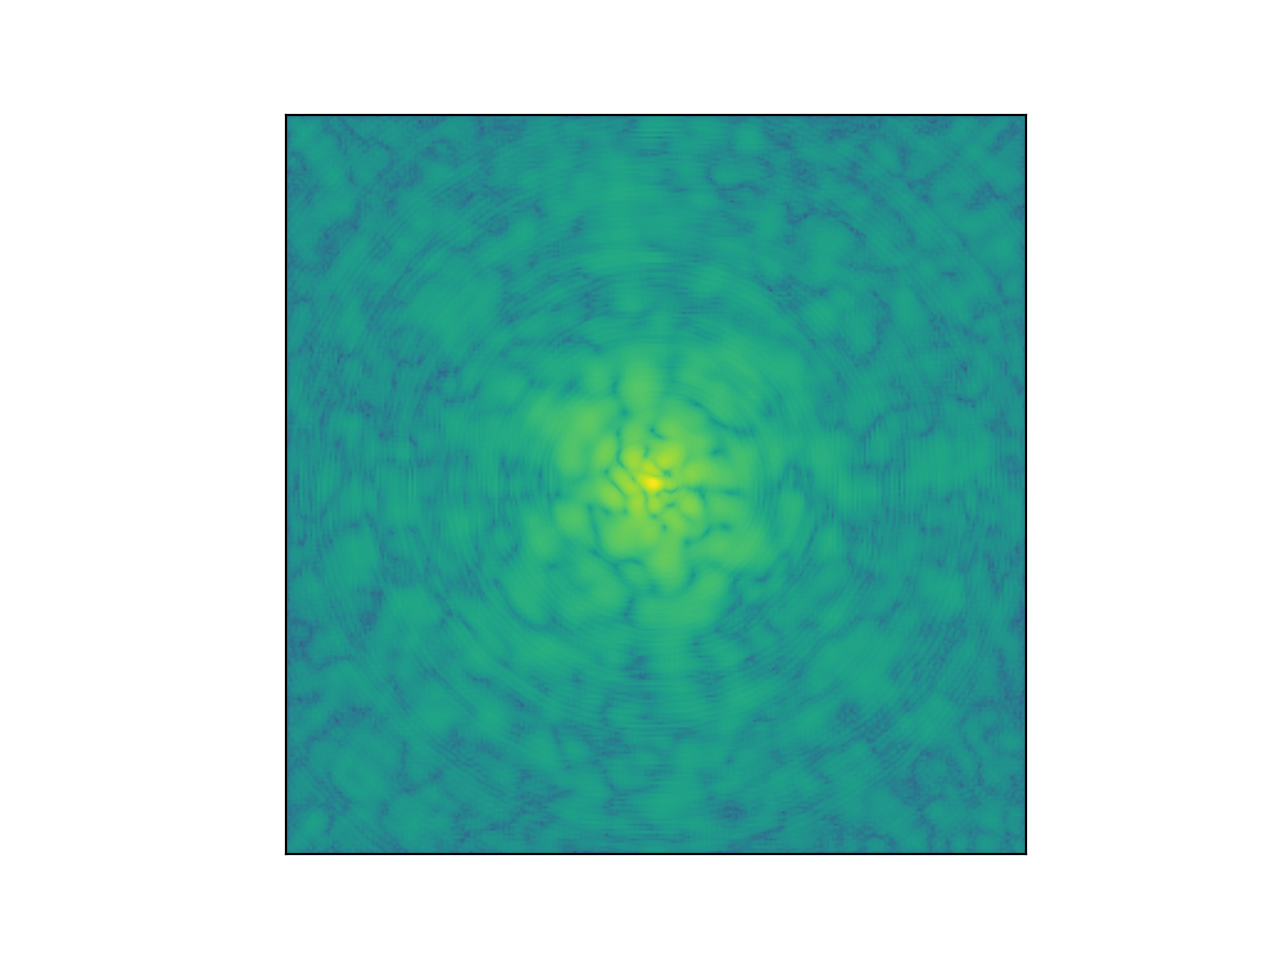
\includegraphics[trim={3cm 0 0 0},scale=0.5]{single_light_plane_107.png}
\endminipage
\caption{Log density distributions through the centre of the simulation region for the $\mathrm{m}_0$ case. From left to right z = 99.5, z = 96.5, and z = 1.5.}\label{fig:contours_light}
\end{figure}


\begin{figure}[!htb]
\minipage{.32\textwidth}
  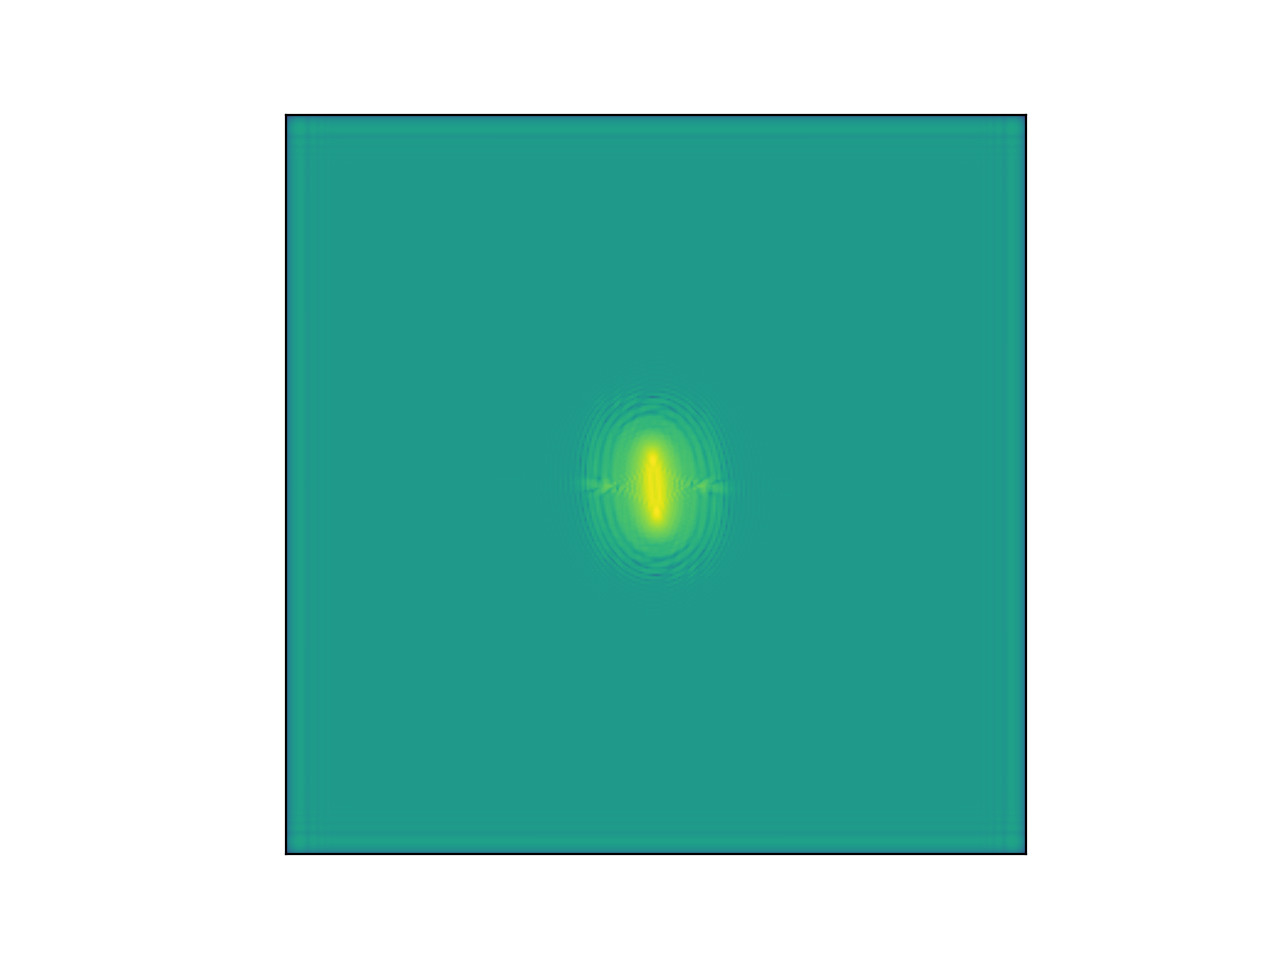
\includegraphics[trim={3cm 0 0 0},scale=0.5]{single_mid_plane_1.png}
%   \caption{A really Awesome Image}\label{fig:awesome_image1}
\endminipage\hfill
\minipage{0.32\textwidth}
  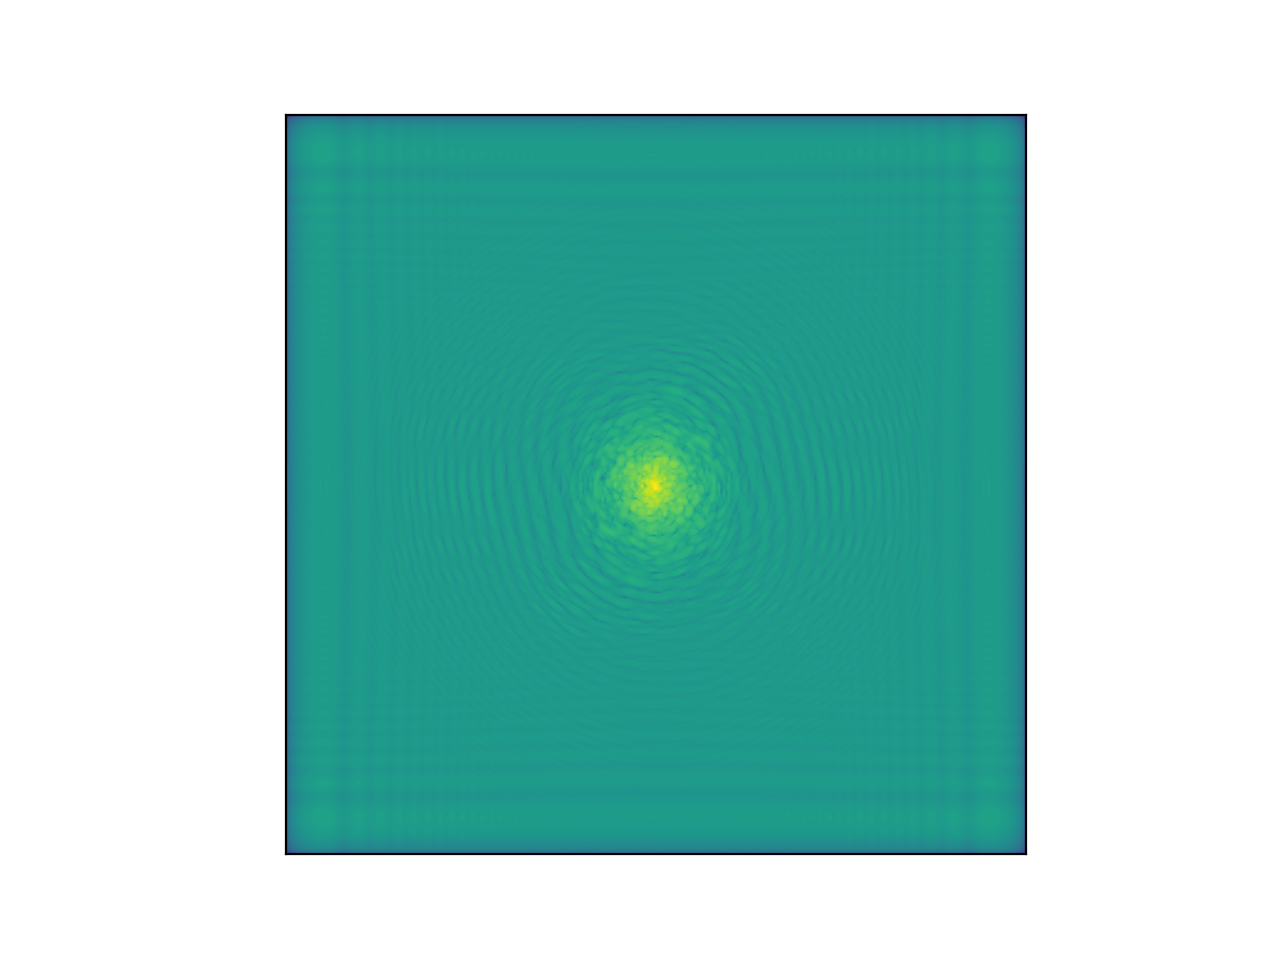
\includegraphics[trim={3cm 0 0 0},scale=0.5]{single_mid_plane_7.png}
%   \caption{A really Awesome Image}\label{fig:awesome_image2}
\endminipage\hfill
\minipage{0.32\textwidth}%
  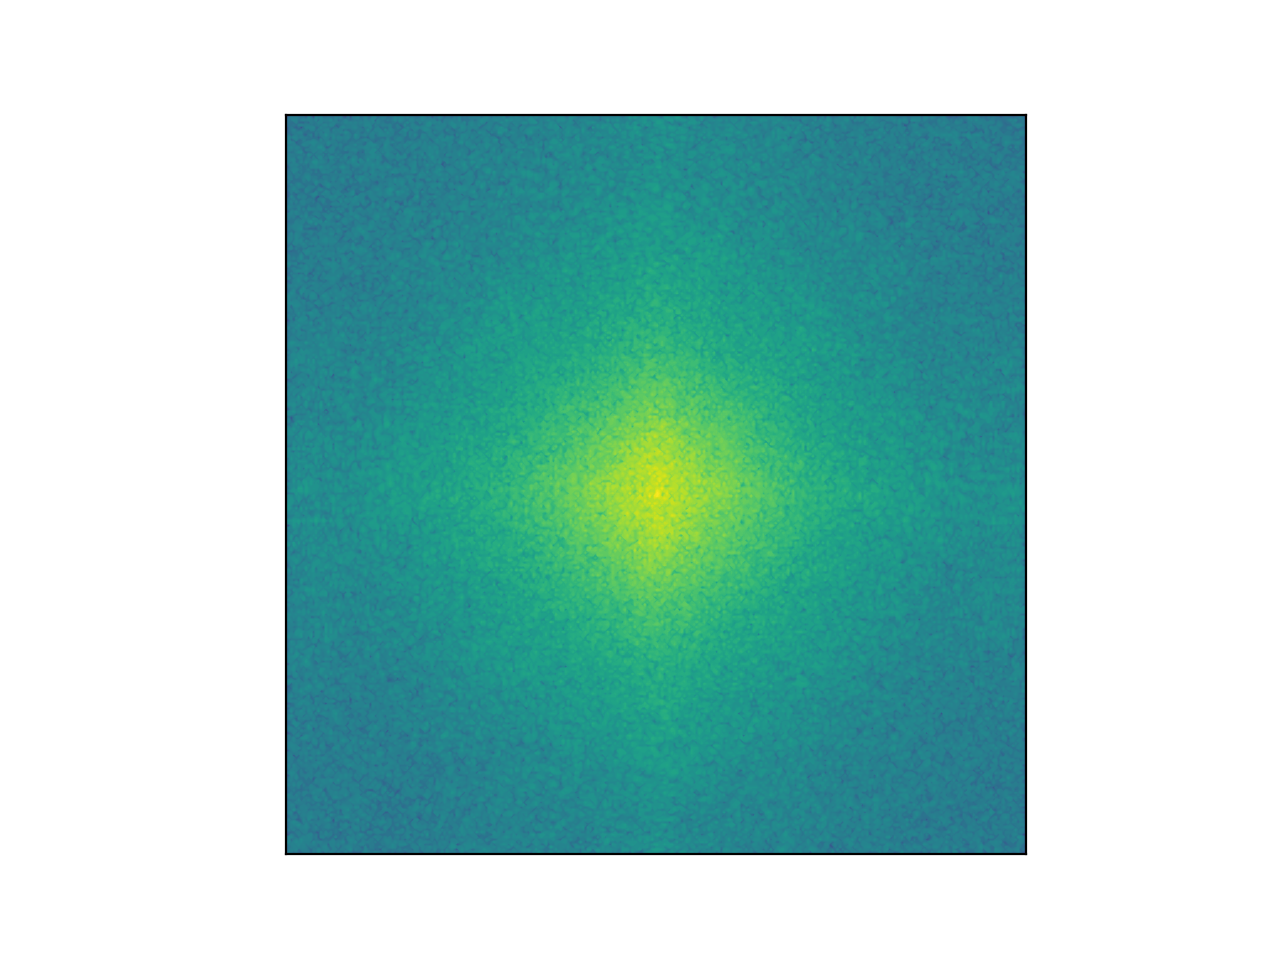
\includegraphics[trim={3cm 0 0 0},scale=0.5]{single_mid_plane_107.png}
%   \caption{A really Awesome Image}\label{fig:awesome_image3}
\endminipage
\caption{Log density distributions through the centre of the simulation region for the $10 \mathrm{m}_0$ case. From left to right z = 99.5, z = 96.5, and z = 1.5.}\label{fig:contours_mid}
\end{figure}


In order for the initial ellipsoidal overdensities to evolve into relaxed halos, mass is expelled from the centre of the simulation through a gravitational cooling mechanism \cite{Seidel:1993zk, Guzman:2006yc}. In this way, excess kinetic energy is removed, allowing the formation of a compact solitonic core. The gravitational cooling mechanism can be viewed as arising from the scattering of the interference fringes generated during the collapse of the overdensity \cite{Arvanitaki:2019rax}. Hence, we expect an exaggerated overall mass loss in cases where the interference fringes are more pronounced, that is, a smaller ULDM particle mass. As time goes on, we expect the mass ejection to become less energetic, enabling a final stable configuration to arise. Indeed, Figure \ref{fig:grav_cool} demonstrates that the gravitational cooling process for the $\mathrm{10m}_0$ case (orange line) terminates at relatively high redshift, with the integrated mass within the simulation region thereafter remaining almost constant. Meanwhile, the $\mathrm{m}_0$ case (blue line) demonstrates a much greater overall mass decrease, extended over a greater time frame. At z = 1.5, the rate of mass loss only just begins to approach zero. Included also in Figure $\ref{fig:grav_cool}$ for reference is the total mass as a function of redshift for $\mathrm{25m}_0$. In this case, only a small proportion of the total mass is lost, occuring at high redshift. Hence, we see that the gravitational cooling mechanism quickly becomes irrelevant at high ULDM particle mass, as the de Broglie wavelength decreases. 

\begin{figure}[!htb]
\minipage{.45\textwidth}
  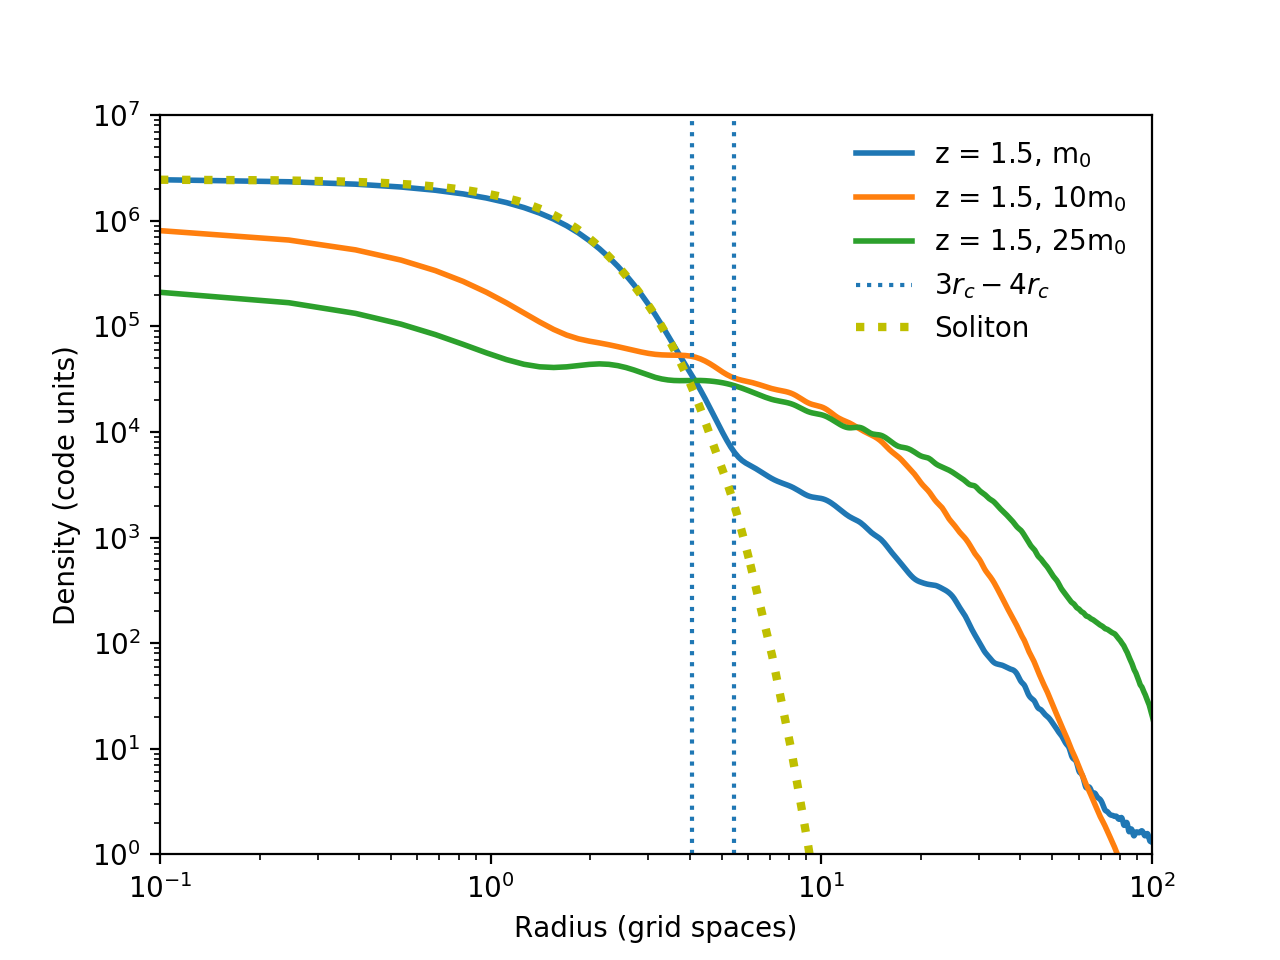
\includegraphics[trim={1.5cm 0 1cm 0},scale=0.55]{final_profile_comparison.png}
  \caption{Spherical average density profiles at z = 1.5 for varying ULDM particle mass. The solitonic core is clearly visible for mass $\mathrm{m}_0$.}\label{fig:final_prof}
\endminipage\hfill
\minipage{0.45\textwidth}
  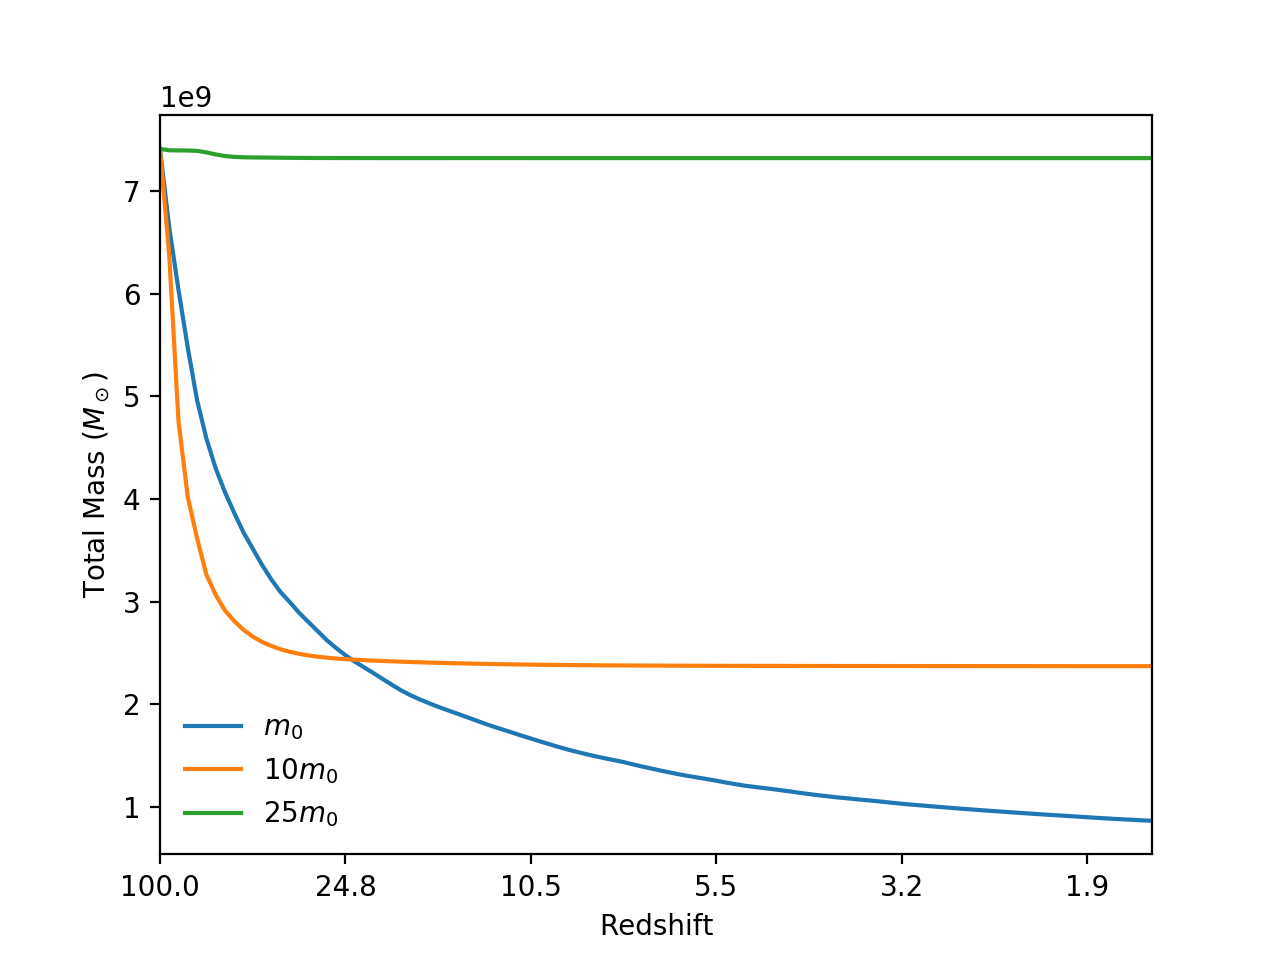
\includegraphics[trim={1.6cm 0 0 0.8cm},scale=0.55]{mass_loss_by_ULDM_mass.png}
  \caption{Total mass as a function of redshift for differing ULDM particle mass. Mass is lost due to gravitational cooling.}\label{fig:grav_cool}
\endminipage\hfill
\end{figure}

Figure \ref{fig:final_prof} demonstrates the spherical averaged density profiles for $\mathrm{m}_0$, $\mathrm{10m}_0$, and $\mathrm{25m}_0$ at z = 1.5. The solitonic core formed in the $\mathrm{m}_0$ case is clearly visible, and is plotted against the numerical solitonic profile (yellow dotted line). We see that the solitonic core transitions into a more NFW-like outer halo at approximately three times the core radius $r_c$, where the core radius is defined as the radius at which the density drops to half of the central value. Such a profile is in accordance with predictions of the generic properties of ULDM halos \cite{Veltmaat:2018dfz, Lin:2018whl, Chavanis:2018pkx}. For the cases in which the particle mass is higher ($\mathrm{10m}_0$, $\mathrm{25m}_0$), the characteristic solitonic core of ULDM is much less well-defined. This change in profile behaviour is consistent with the fact that as ULDM particle mass is increased, we recover the CDM limit in which halos can be described by the semi-analytic NFW profile. 

\section{Dependence of gravitational cooling rates on ellipticity}\label{sec:flattening}

In the previous section, we demonstrated that gravitational cooling arises due to the wave-like properties of the ULDM field. As a consequence, a smaller ULDM particle mass corresponds to a more pronounced gravitational cooling effect. In this section, we demonstrate that the mass loss through gravitational cooling is also dependent upon the shape of the overdensity. To demonstrate this, we set up three overdensities defined by Equation \ref{eq:ellipse}. Again we choose R to be 100 grid spaces, and a constant density within the ellipsoid of 2500 grid units. We consider ellipsoids in which two of the principal axes are of equal length, with the third axis shorter. In this case, we can define the flattening parameter of the ellipsoid as follows:
\begin{equation}
    f = \frac{a-c}{a},
\end{equation}
where a is the length of the two larger axes, and b is the length of the third, smaller axis. We consider three cases, namely $\{a = b = 2, c = 2\}$, $\{a = b = 5/2, c = 32/25\}$, and $\{a = b = 3, c = 8/9\}$. These ellipsoids all have the same volume, but flattening parameters of $f = 0$, $f = 0.5$, and $0.7$, respectively. We find that The effect of gravitational cooling is more pronounced for the spherical configuration, decreasing as the initial overdensity is flattened. This is consistent with the idea that for very flat configurations, approaching the Zel'dovich pancake, collapse largely occurs along the two longest axes only, thereby decreasing the ejection of excess kinetic energy arising from interference patterns created during collapse along the shortest axis. The effect of flattening the overdensity on the rate of gravitational cooling is demonstrated in Figure \ref{fig:mass_loss_flattening}. Despite varying initial overdensity shape, the final relaxed profiles are largely spherically symmetric, with the inner region well approximating the theoretical soliton profile. The relaxed density profiles are shown in Figure \ref{fig:final_profiles_flattening}. We note that while the final halo masses differ in all cases, for $f = 0.5$ and $f = 0.7$, the solitonic region is almost identical, with the difference in mass being accounted for by the incoherent outer halo. This suggests a degree of variability in the theoretical core-halo mass relation \cite{Schive:2014dra, Bar:2018acw}. We will return to this point in Section \ref{sec:core-halo}. 

\begin{figure}[!htb]
\minipage{0.45\textwidth}
  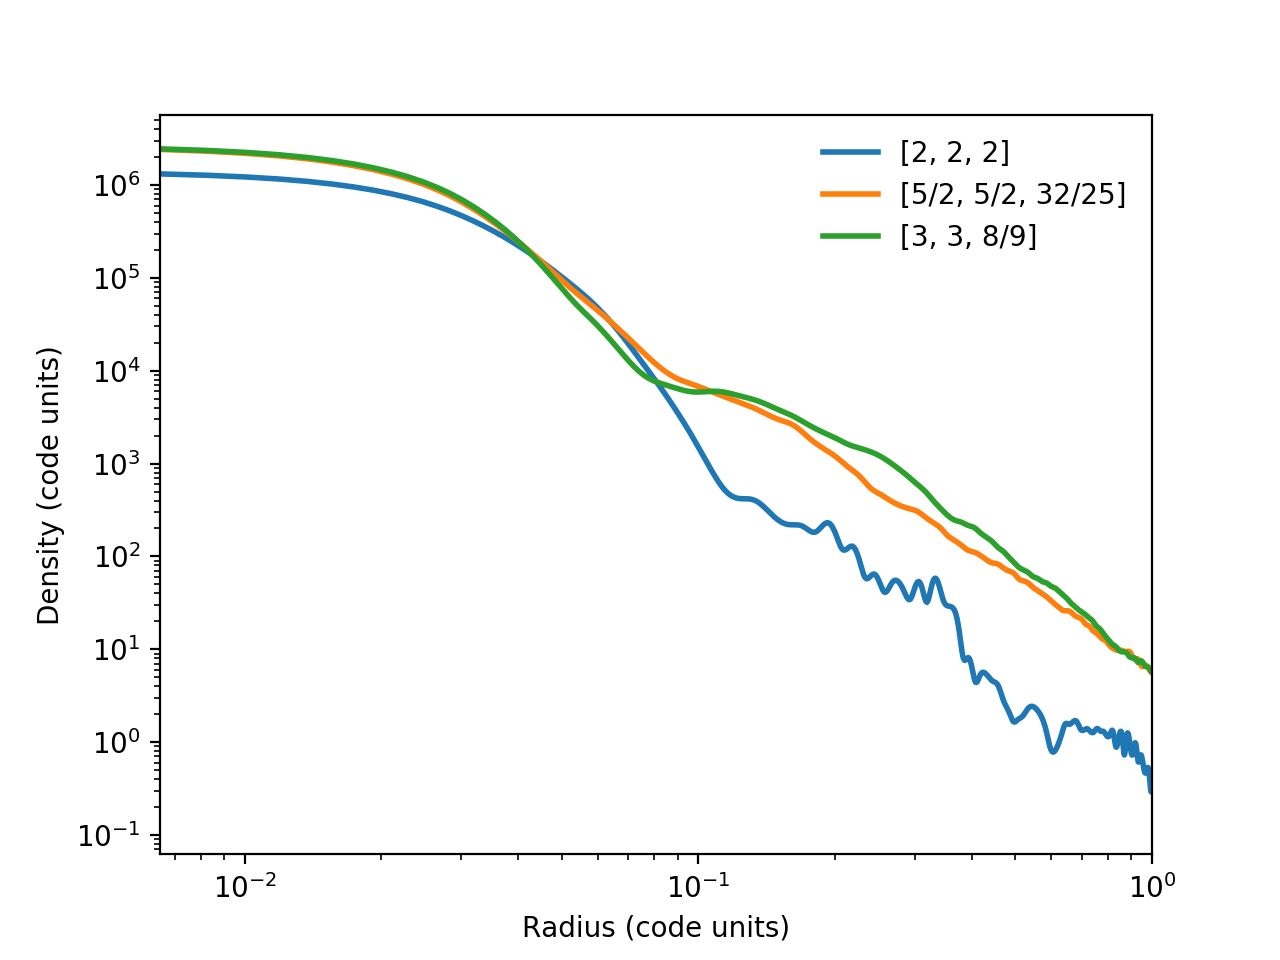
\includegraphics[trim={1.6cm 0 0 0cm},scale=0.55]{final_profiles_flattening.png}
  \caption{Final spherically averaged density profiles for varying initial flattening parameters, $f = \{0, 0.5, 0.7\}$.}\label{fig:final_profiles_flattening}
\endminipage\hfill
\minipage{.45\textwidth}
  \includegraphics[trim={1.5cm 0 1cm 0cm},scale=0.55]{mass_loss_flattening.png}
  \caption{Mass loss due to gravitational cooling for varying flattening parameters, $f = \{0, 0.5, 0.7\}$.}\label{fig:mass_loss_flattening}
\endminipage\hfill
\end{figure}

\section{Effect of angular momentum on overdensity collapse}\label{sec:rotation}

In this section, we augment the previous simulation setups by adding a varying phase parameter in order to generate angular momentum in the initial overdensities. To do this, we first create a gaussian profile for the magnitude of the phase parameter, concentric with the initial overdensity. The Gaussian profile is determined by three parameters, $\{a, \bold{b}, c\}$ through

\begin{equation}\label{eq:gauss}
    f(\bold{x}) = a\exp\left(-\frac{(\bold{x}-\bold{b})^2}{2c^2}\right)    
\end{equation}

We then distort this spherical gaussian profile to create an ellipsoidal profile with the same three axis parameters as the overdensity itself. However, we offset the orientations of the two ellipsoids by some non-zero angle. We then assign a phase $\theta$ to each field point, with the magnitude of the phase determined by the distorted Gaussian magnitude $f(\bold{x})$ at that grid position. That is,  

\begin{equation}
    \psi \rightarrow \psi \times \exp(i\theta),
\end{equation}
\\
where $\theta$ is determined by the distorted Gaussian. Because the velocity of the ULDM field is given by $\bold{v} = \bold{\nabla} \theta$, this process imparts rotational velocity to the original ellipsoidal overdensity. By varying the magnitude of the Gaussian parameter $a$ in Equation \ref{eq:gauss}, we can change the magnitude of the angular momentum of the overdensity.

We note that because we allow mass to be ejected from the simulation grid, we do not conserve angular momentum. Furthermore, the periodic boundary conditions of {\sc PyUltraLight} do not allow for conservation of  angular momentum by definition. Thus, the study of the intrinsic rotation of the field allows for an understanding of the distribution of angular momentum during overdensity collapse, but cannot yield a comprehensive quantitative analysis.

To initialise the simulation, we use the same setup as described in Section \ref{sec:collapse}, namely, a resolution of $300^3$, $R = 100$ grid spaces and the parameters of Equation \ref{eq:ellipse} defined as $\{a = b = 3, c = 8/9\}$. The side length of the simulation region is set to $10a(t)$ code units and the density within the ellipsoid is set to $\rho = 2500$ code units.
We then add the distorted Gaussian phase field, offset from the overdensity by an angle of 1 radian. We examine two cases, the first of which employs the Gaussian parameters $a = 2.5$, $c = 0.5$, while in the second case we choose $a = 10$, $c = 0.5$. We run the simulation from $z = 100$ to $z = 1.5$.

In the first case, we find that while the overdensity rotates slowly, the rate of rotation is sufficiently small that the overdensity is still able to collapse. In the latter case, however, we find that the high rotational velocity overcomes the gravitational attraction and the overdensity is torn apart at early times. We demonstrate the difference in the field configurations at $z=96$ for the two cases in Figures \ref{fig:rot_comp_2_5} and \ref{fig:rot_comp_2_5}.

\begin{figure}[!htb]
\minipage{.45\textwidth}
  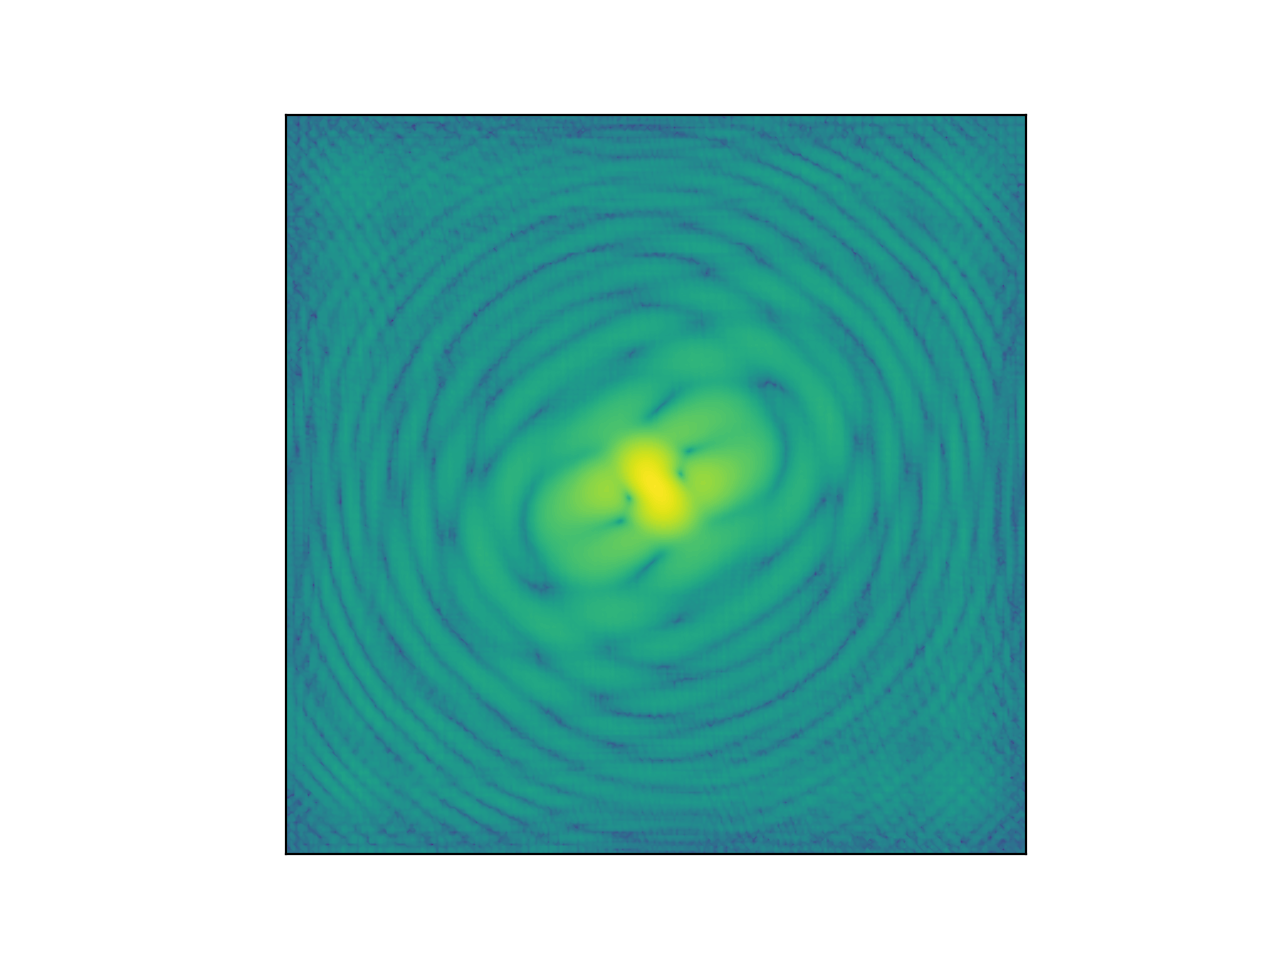
\includegraphics[trim={2cm 0 1cm 0cm},scale=0.55]{rot_comp_2_5.png}
  \caption{Log-scaled density distribution through the centre of the field across the centre of the axis of rotation for Gaussian parameter $a = 2.5$ at $z=96$. a central collapsed region is visible.}\label{fig:rot_comp_2_5}
\endminipage\hfill
\minipage{.45\textwidth}
  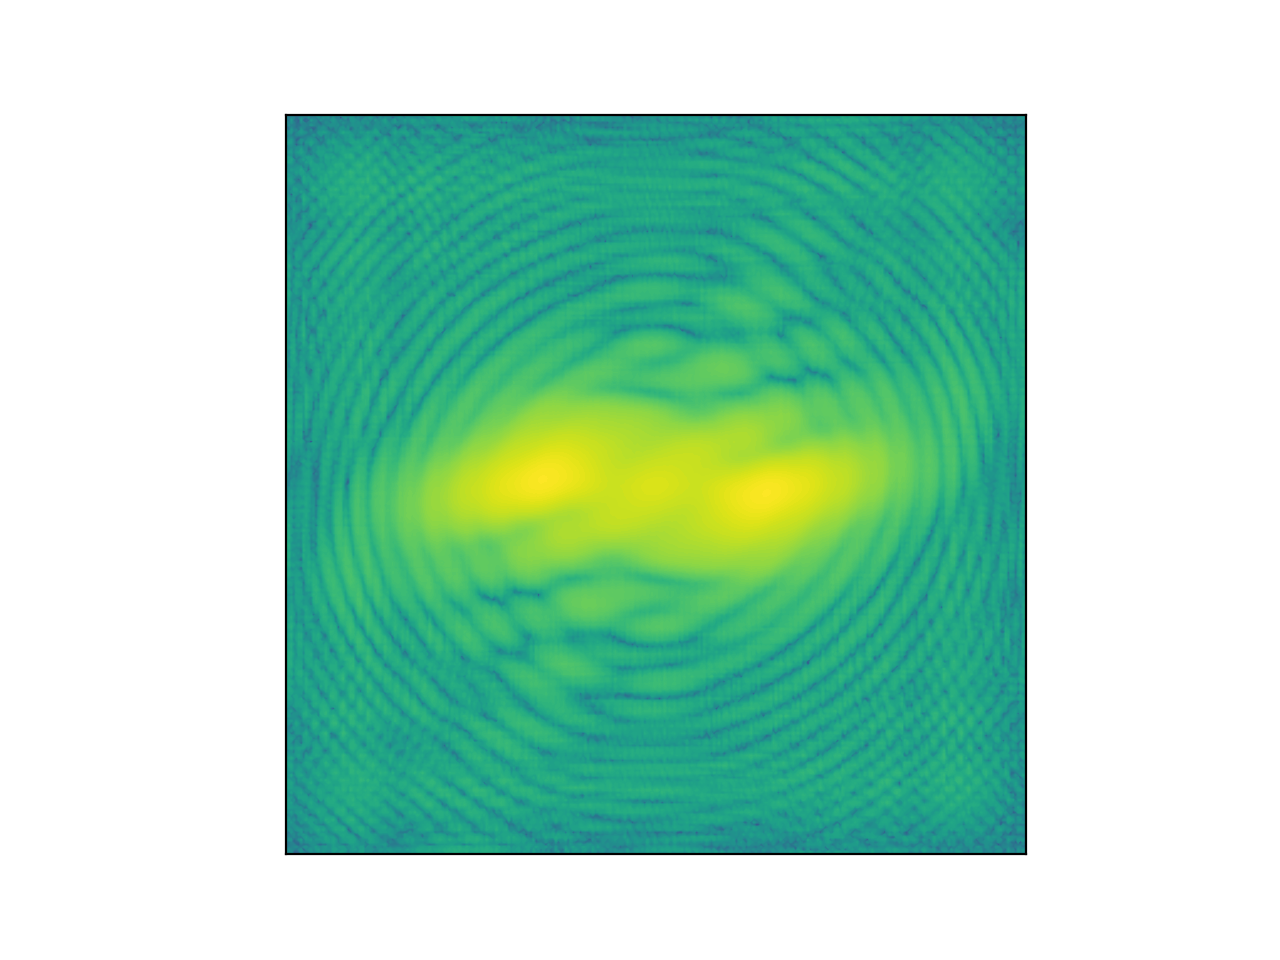
\includegraphics[trim={2cm 0 1cm 0cm},scale=0.55]{rot_comp_10.png}
  \caption{Log-scaled density distribution through the centre of the field across the centre of the axis of rotation for Gaussian parameter $a = 10$ at $z=96$. Here the initial overdensity is torn apart.}\label{fig:rot_comp_10}
\endminipage\hfill
\end{figure}

In the case of low rotational velocity ($a = 2.5$) we consider the component of the angular momentum along the axis of rotation at $z = 96$ and $z = 1.5$. We plot this for the central $100^2$ grid points of the plane through the centre of the simulation in Figures \ref{fig:ang_mom_early} and \ref{fig:ang_mom_complete}. In Figure \ref{fig:ang_mom_early} we can clearly see the angular momentum distribution characteristic of a uniformly rotating central overdensity. At late times, however, much of the angular momentum has been radiated away through gravitational cooling. Nevertheless, rotation appears to persist within the collapsed core, which is now slightly off-centre. As the simulation progresses, we see movement in the position of the core, seemingly affected by residual angular momentum in the incoherent outer halo. A lack of resolution in the core of the final halo makes a quantitative study of its angular momentum difficult, though this simulation serves as a motivation for further study of rotating solitonic cores within ULDM halos. We confirm that the central region of the collapsed halo does in fact follow a spherical solitonic profile, as illustrated in Figure \ref{fig:rot_complete}.


\begin{figure}[!htb]
\minipage{.45\textwidth}
  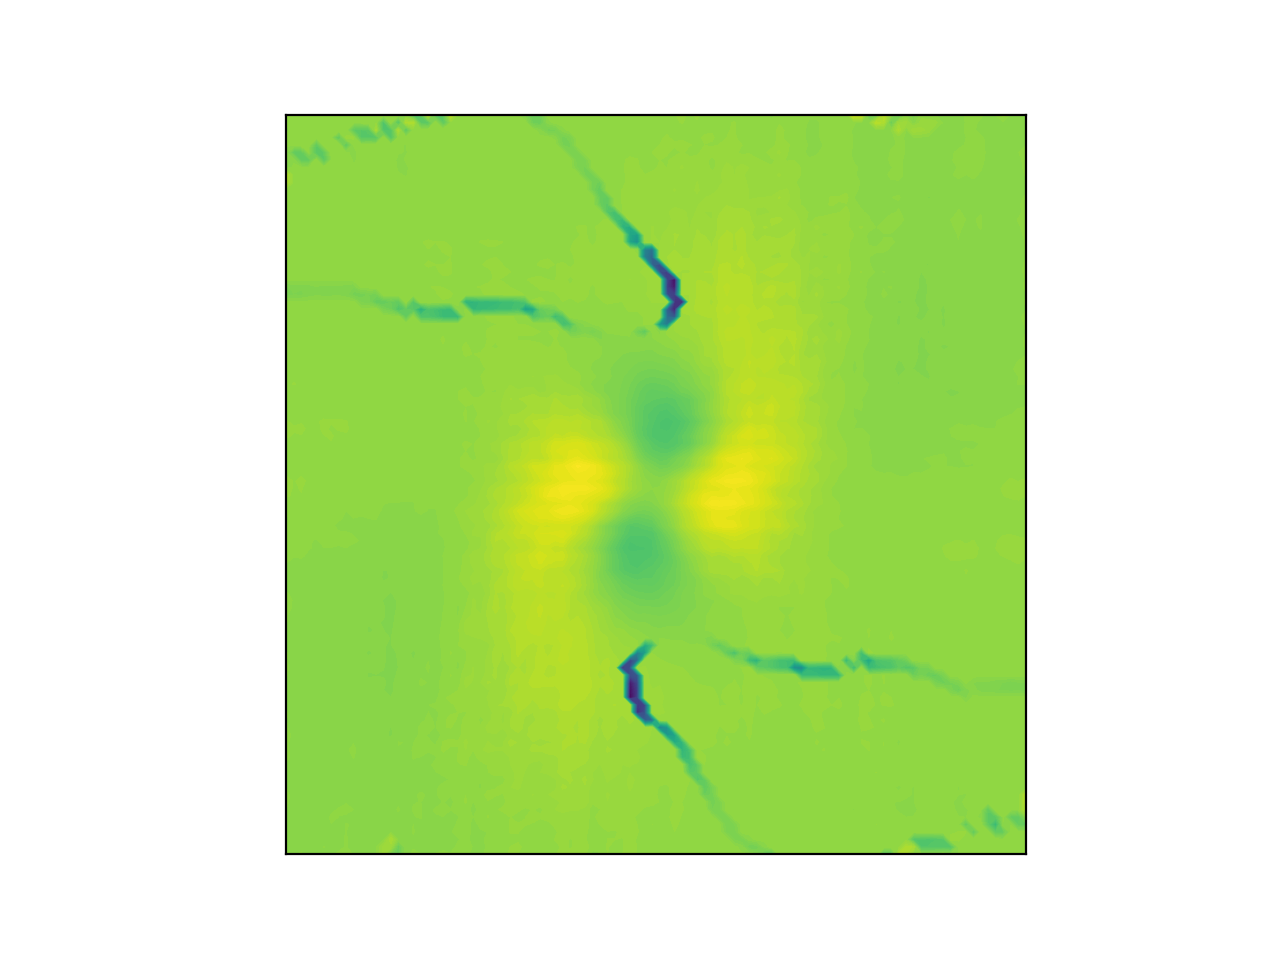
\includegraphics[trim={2cm 0 1cm 0cm},scale=0.55]{ang_mom_early.png}
  \caption{Angular momentum component along the axis of rotation for $a = 2.5$, $z = 96$.}\label{fig:ang_mom_early}
\endminipage\hfill
\minipage{.45\textwidth}
  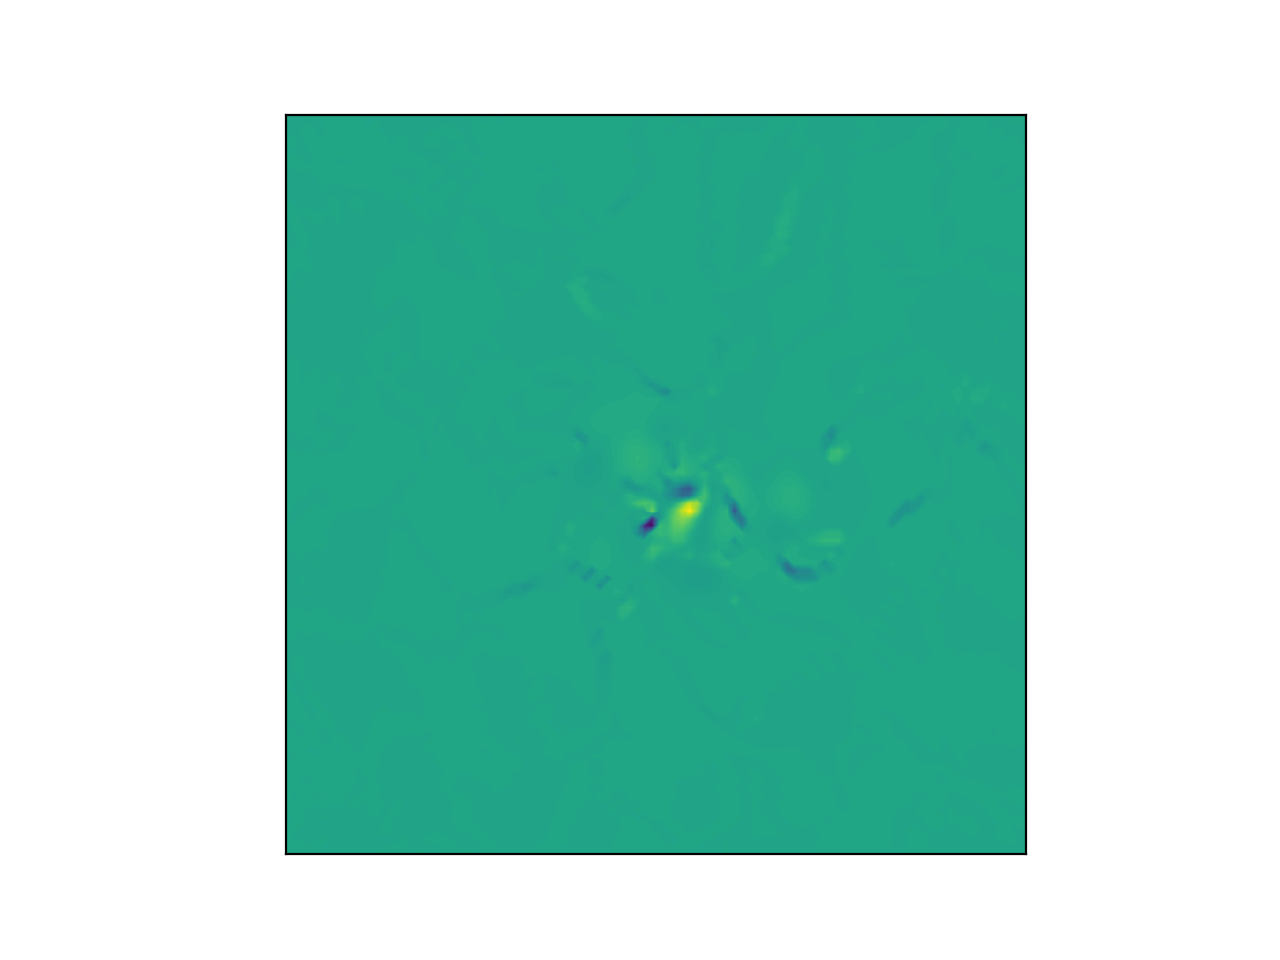
\includegraphics[trim={2cm 0 1cm 0cm},scale=0.55]{ang_mom_complete.png}
  \caption{Angular momentum component along the axis of rotation for $a = 2.5$, $z = 1.5$.}\label{fig:ang_mom_complete}
\endminipage\hfill
\end{figure}

\begin{figure}[!htb]
\centering
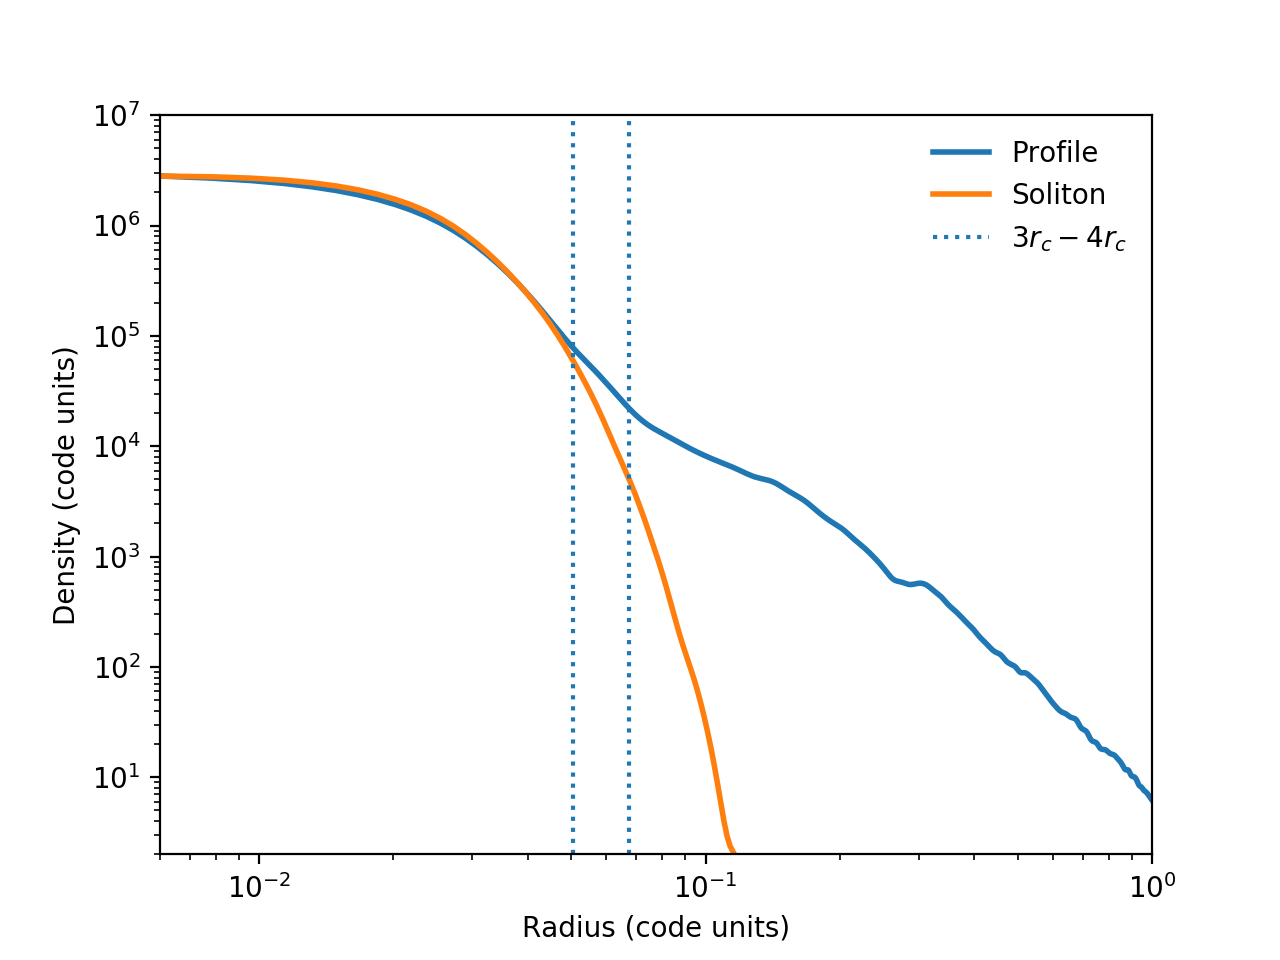
\includegraphics[trim={0 0 0 0},scale=0.6]{rot_complete.png}
\caption{Final relaxed profile ($z = 1.5$) obtained through collapse of the rotating overdensity characterised by Gaussian parameter $a = 2.5$.}\label{fig:rot_complete}
\end{figure}


\section{Apparent variability in the core-halo mass relation}\label{sec:core-halo}

In this section, we present a case in which the theoretical core-halo relation \cite{Schive:2014dra, Bar:2018acw} appears to be violated. We conduct two simulations of overdensity collapse. In the first simulation, we use the same initial conditions as used in \ref{sec:collapse}, namely, an ellipsoidal overdensity defined by $R = 100$ grid spaces and $\{a = b = 3, c = 8/9\}$ in a box of side length $10 a(t)$ code units. The internal density of the ellipsoid is set to $2500$ code units. In the second simulation, all parameters remain the same except $R$, which in this case is set to $R = 50$ grid spaces. That is to say, we decrease the overall volume of the ellipsoidal overdensity. We do not include rotation in these simulations. We then allow the initial configurations to evolve from $z = 100$ to $z = 1.5$. The mass loss through gravitational cooling and the final spherically-averaged profiles are presented in Figures \ref{fig:mass_loss_comp} and \ref{fig:profiles_comp}, respectively. 

Figure \ref{fig:mass_loss_comp} demonstrates that mass loss rates at the end of both simulations are approaching zero, indicating that the profiles have stabilised\footnote{We note, however, that it is difficult to define the point at which a halo is completely `stabilised', especially if such a halo exists within a dynamic environment.}.The final total mass in the $R = 100$ case is roughly twice that of the final mass in the $R = 50$ case. However, inspection of the final density profiles reveals that the solitonic cores in both cases are very similar, with the difference in mass accounted for almost exclusively by the incoherent outer halo. This suggests that a strict core-halo mass relationship is not valid, and motivates further investigation into causes of variation in the the corresponding statistics.

Of course, one naturally expects that the core-halo relationship must break down at some point, given that solitonic profiles widen as mass decreases, such that at some point the core would effectively `envelop' the outer halo. However, in this case we clearly see a well defined core and outer halo, as is to be expected for halos in this mass range (assuming a ULDM particle mass of $10^{-22}\matrm{eV}$ the final cores have masses $1.3\times 10^8 \mathrm{M}_\odot$ and $1.6\times 10^8 \mathrm{M}_\odot$, while the overall spherical halos out to the edge of the simulation regions have masses of $1.0\times 10^9 \mathrm{M}_\odot$ and $2.0\times 10^9 \mathrm{M}_\odot$, respectively). We note, however, that in these contrived simulations of the collapse of isolated ellipsoidal overdensities, the virial mass and radius, as they are typically defined, are somewhat meaningless numbers. This is because the virialisation of a halo is typically defined by the point at which the average internal density is of the order of 200 times the critical density of the universe. In non-cosmological simulations such as these, this does not apply. This motivates a detailed study of the distributions of the kinetic, gravitational, and quantum energies within a ULDM halo, in order to quantitatively ascertain the radius of virialisation. We leave such a study for future work.  

Hence, this section serves as motivation for detailed critical analysis of the physics of the core-halo relationship in ULDM, taking into account environmental variability and internal energy distributions.

%units don't really matter because only thing that's relevant is ratio of dB wavelength to distance scale. So the point is we have a soliton of order 1/n the size of the box, and the halo is only a few times bigger






\begin{figure}[!htb]
\minipage{.45\textwidth}
  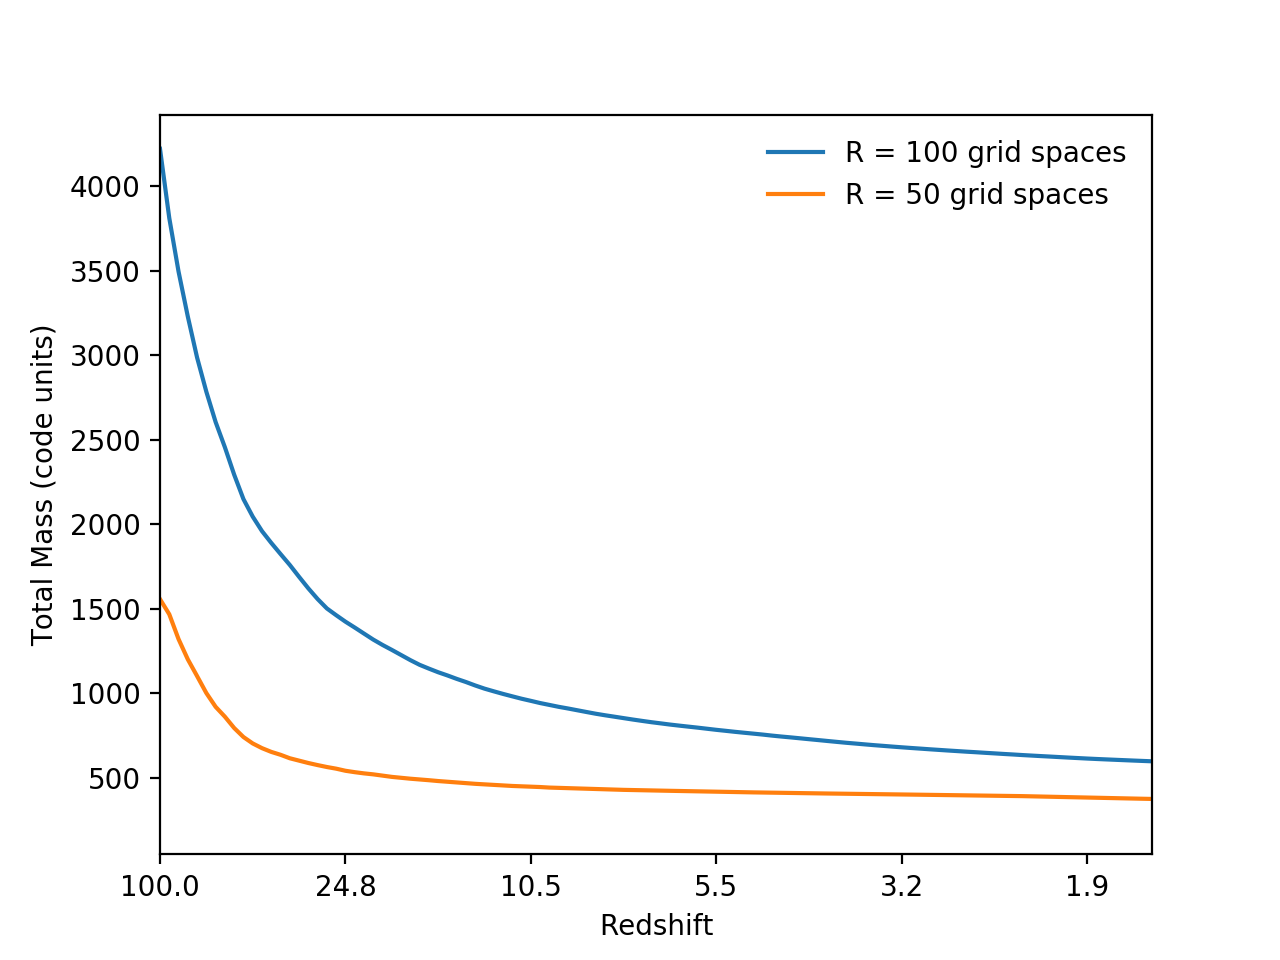
\includegraphics[trim={2cm 0 1cm 0cm},scale=0.55]{mass_loss_comp.png}
  \caption{Mass loss due to gravitational cooling of ellipsoidal overdensities with $R$ parameters $R =100$ and $R = 50$ grid spaces.}\label{fig:mass_loss_comp}
\endminipage\hfill
\minipage{.45\textwidth}
  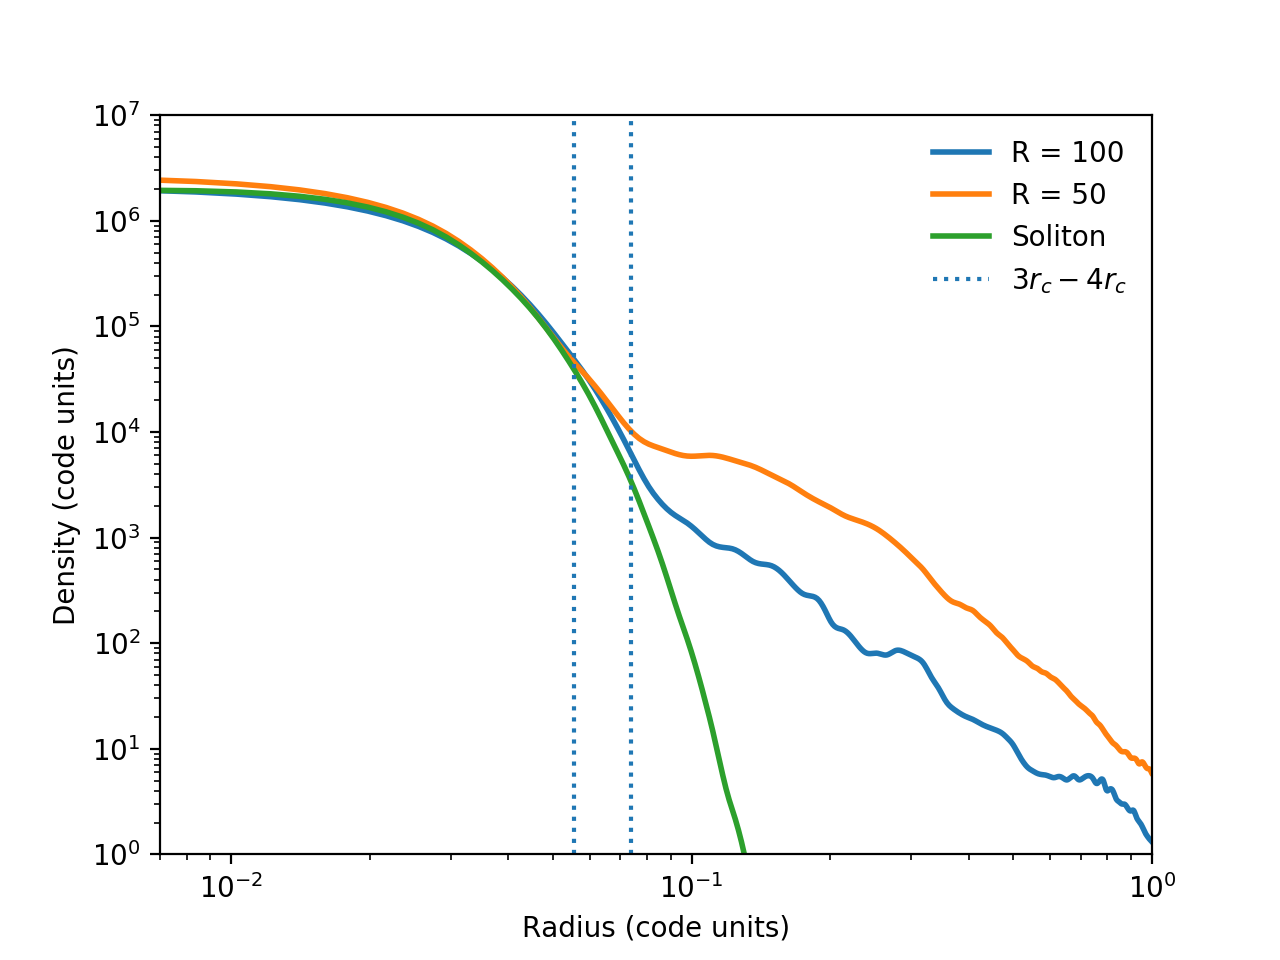
\includegraphics[trim={2cm 0 1cm 0cm},scale=0.55]{profiles_comp.png}
  \caption{Final relaxed profiles for the two simulations, where the difference in the total halo mass is largely accounted for by the outer halo alone.}\label{fig:profiles_comp}
\endminipage\hfill
\end{figure}


\section{Statistics of the traceless tidal tensor in ULDM simulations}\label{sec:stats}

In this section, we perform a proof-of-principle analysis of the statistics of the eigenvalues of the traceless tidal tensor for the simulations of overdensity collapse described in Section \ref{sec:collapse}. This is motivated by the fact that high-resolution cosmological simulations seem to suggest that there may be additional structure present in the filaments of the cosmic web in the ULDM case compared to the CDM case, due to interference effects \cite{Mocz:2019emo}. Such extended anisotropies cannot be completely characterised using the 2-point correlator, and thus it may prove useful to examine the statistics of quantities which preserve information about anisotropy in density distributions, such as the tidal tensor. While we do not suggest that these results can be directly applied to large scale cosmological structure, they serve to motivate the use of such statistical tools as a means by which to quantify the differences between ULDM and CDM density distributions and to possibly constrain the ULDM particle mass. 

\subsection{The traceless tidal field in the principal axis frame}\label{sec:TTT}

From the density fields output by the {\sc PyUltraLight} simulation tool, we construct the traceless tidal tensor at each grid point. To do this, we first compute the dimensionless overdensity field:
\begin{equation}
    \delta(\mathrm{\mathbf{x}}) = \frac{\rho(\mathrm{\mathbf{x}})-\Bar{\rho}}{\bar{\rho}}, 
\end{equation}
where $\bar{\rho}$ is the average density throughout the simulation volume. We then take the Fourier transform to obtain the dimensionless density contrast in Fourier space, $\delta(\mathrm{\mathbf{k}})$. From here we can calculate the peculiar gravitational field from the Poisson equation, and finally compute the tidal tensor as the Hessian of the peculiar gravitational potential. In Fourier space we have
\begin{equation}
    \phi(\mathrm{\mathbf{k}}) = k^{-2}\delta(\mathrm{\mathbf{k}}), \qquad T_{ij}(\mathrm{\mathbf{k}}) = k_{i}k_{j}\phi(\mathrm{\mathbf{k}}).
\end{equation}
At each point, the dimensionless density contrast is given by the trace of the tidal tensor. Therefore, in order to isolate the tidal effects, we compute the traceless tidal tensor:
\begin{equation}
    \Tilde{T}_{ij}(\mathrm{\mathbf{k}}) = T_{ij}(\mathrm{\mathbf{k}}) - \frac{\delta(\mathrm{\mathbf{k}})}{3}\mathbb{I}_{ij}.
\end{equation}
Finally we perform an inverse Fourier transform to obtain the traceless tidal tensor in real space. We then randomly select a sample of 15,000 points from the simulation grid at which to diagonalise the tidal tensor, storing the eigenvalues ($\lambda_1$, $\lambda_2$, $\lambda_3$) and unit eigenvectors ($\mathrm{\mathbf{e}}_1$, $\mathrm{\mathbf{e}}_2$, $\mathrm{\mathbf{e}}_3$) for further analysis. We label the eigenvalues such that $\lambda_1 >\lambda_2 > \lambda_3$. Because these are the eigenvalues of the\textit{traceless} tensor, we also have $\lambda_1>0$ and  $\lambda_3 < 0$, while $\lambda_2$ may be either positive or negative.

To compute the correlation functions, we consider the principal axis frame defined by $\mathrm{\mathbf{e}}_1$, $\mathrm{\mathbf{e}}_2$, $\mathrm{\mathbf{e}}_3$ for every sample point $\mathrm{\mathbf{x}}$. We consider pairs of points $\mathrm{\mathbf{x}}$ and $\mathrm{\mathbf{x}}+\mathrm{\mathbf{r}}$, where $\mathrm{\mathbf{r}}$ is the separation vector in the principal axis frame of $\mathrm{\mathbf{x}}$. We convert $\mathrm{\mathbf{r}}$ into spherical polar coordinates $r, \theta, \varphi$ and finally define 
\begin{equation}
    \xi_{\lambda_i}(r, \theta, \varphi) = \langle\lambda_i(\mathrm{\mathbf{x}})\lambda_i(\mathrm{\mathbf{r+x}})\rangle.
\end{equation}
We must of course specify a convention for our definition of $\theta$ and $\varphi$. In this case we choose 
\begin{align}
    r &= \sqrt{e_3^2+e_2^2+e_1^2}\nonumber\\
    \theta &= \tan^{-1}\left(\frac{e_2}{e_3}\right)\nonumber\\
    \varphi &= \cos^{-1}\left(\frac{e_1}{r}\right)\nonumber
\end{align}
We will consider both $\xi_{\lambda_i}(r)$ and $\xi_{\lambda_i}(r,\varphi)$, whereby in the former case the average is taken over all separation vectors in differential bins $[r, r+dr]$, and in the latter case the averages are further separated into differential bins $[\varphi, \varphi + d\varphi]$.

\subsection{Probability distributions of the eigenvalues of the traceless tidal tensor}\label{sec:probs}

We have thus far seen striking visual differences arise during the collapse of overdensities for differing ULDM particle masses (Figures \ref{fig:contours_light} and \ref{fig:contours_mid}). These differences occur because of interference between the wavefronts of the massive scalar field, ejected during the gravitational cooling process. Wavefronts and their interference patterns are intrinsically anisotropic structures. Thus, it is of interest to analyse such structures using statistical tools designed to take anisotropy into account. As described in Section \ref{sec:TTT}, the traceless tidal tensor at each point in a density field gives the deformation of the corresponding volume element relative to purely spherical expansion or collapse. It is therefore an ideal tool to characterise fields in which structures possessing directional dependence arise. 

In particular, rather than using the traditional isotropic 2-point matter correlation function to analyse density distributions, we can instead examine the 2-point correlation functions of the eigenvalues of the traceless tidal tensor in its principal axis frame, as well as the probability distributions of the eigenvalues. The principal axis frame at each point is defined by the eigenvectors of the traceless tidal field, where the maximal compression of a volume element occurs along the direction of the eigenvector associated with the largest eigenvalue. Hence, this method preserves information about the anisotropy of the local gravitational field. 

Before analysing the correlation functions of the eigenvalues of the traceless tidal tensor, we will examine their overall probability distributions. We will consider the density fields arising during the collapse of ULDM overdensities with differing particle mass, as described in the previous section. In general, we expect the presence of repeated anisotropic structures such as wavefronts to induce peaks in the probability distributions of the eigenvalues, as in such cases there will be a number of volume elements exhibiting the same characteristic anisotropic deformation. In Appendix \ref{app:prob_distro_eg} we demonstrate this effect using artificial density distributions. 

We consider again the simulations described in Section \ref{sec:collapse}, the results of which are illustrated in Figures \ref{fig:contours_light} to \ref{fig:grav_cool}. Figure \ref{fig:singles_distros} shows the probability distributions of the eigenvalues of the traceless tidal tensor for z = 96.5 and z = 1.5, where at each redshift we consider density distributions for both $\mathrm{m}_0$ and $\mathrm{10m}_0$. Because the traceless tidal field was computed for 15,000 randomly chosen points within the simulation grid, there are a total of 45,000 data points from which to construct the probability distributions of the three eigenvalues. Because we have a finite number of samples, we must choose a smoothing method to obtain a continuous distribution. In this case, we divide the eigenvalue range $\{-3,+3\}$ into 1000 bins, tallying the number of points which fall into each bin. We represent the outcome of this procedure using the scattered points in Figure \ref{fig:singles_distros}. In order to gauge the presence of peaks in the distribution, we overlay these points with a best-fit cubic spline interpolation. The degree of smoothing will of course affect the visible level of substructure, however we note that the smoothing procedure applied here is sufficient to identify qualitative differences in the probability distributions of the $\mathrm{m}_0$ and $\mathrm{10m}_0$ cases. In particular, we see that at high redshift (z = 96.5), the eigenvalue distribution for the lower ULDM mass case is visibly more uneven than that of the higher ULDM mass case. We see the presence of distinct peaks, indicative of extended anisotropic structures. By contrast, the probability distributions at high redshift are much more similar in appearance, accounting for the fact that distinct elongated wavefronts are no longer present in the relaxed halos. 

\begin{figure}[!htb]

\minipage{0.5\textwidth}
  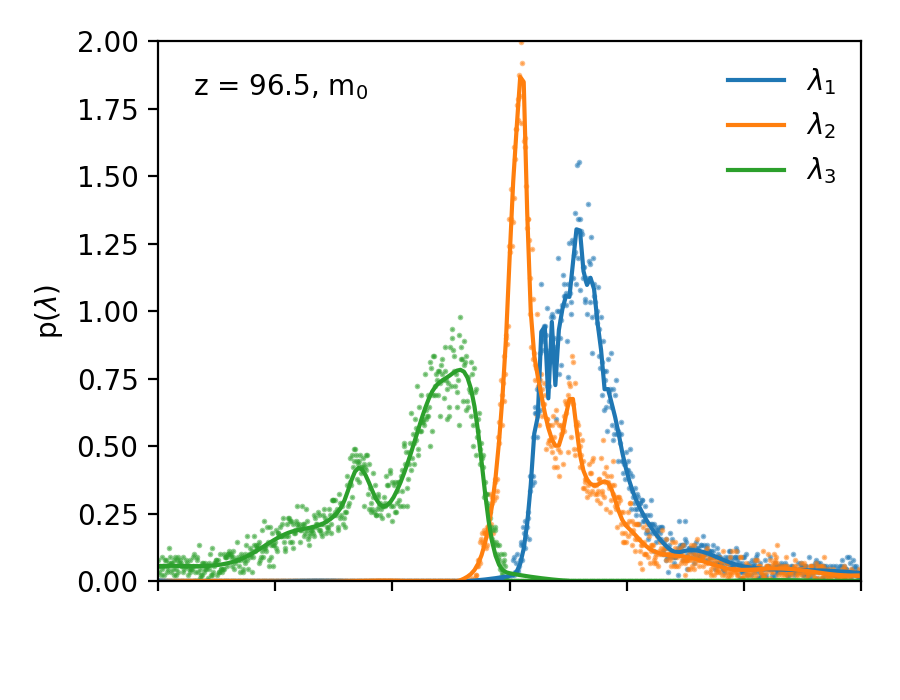
\includegraphics[trim={1cm 0 0 0},scale=0.8]{distro_single_light_7.png}
%   \caption{A really Awesome Image}\label{fig:awesome_image2}
\endminipage\hfill
\minipage{0.5\textwidth}%
  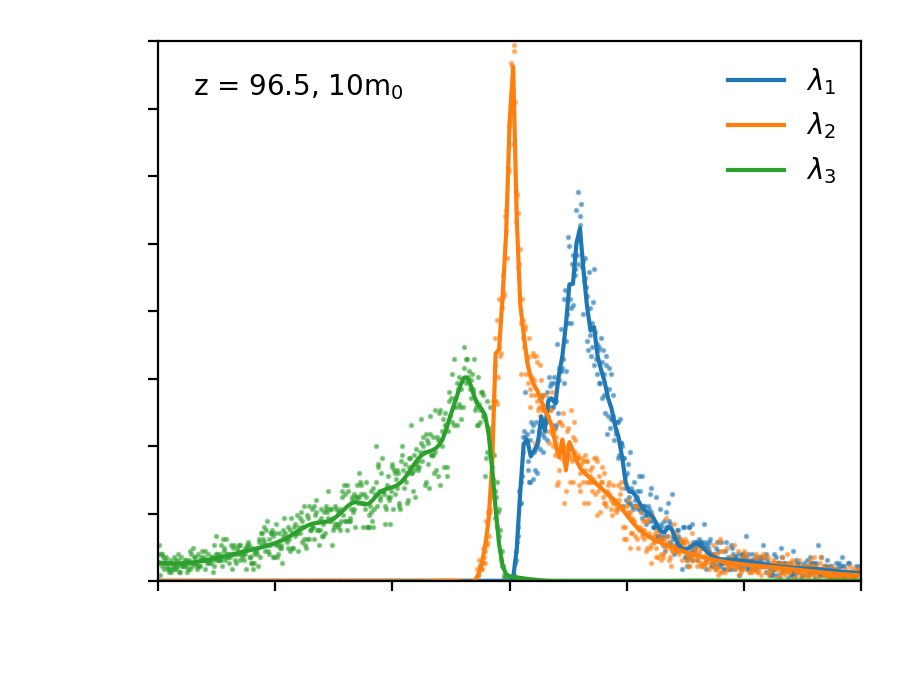
\includegraphics[trim={1cm 0 0 0},scale=0.8]{distro_single_mid_7.png}
%   \caption{A really Awesome Image}\label{fig:awesome_image3}
\endminipage

\minipage{0.5\textwidth}
  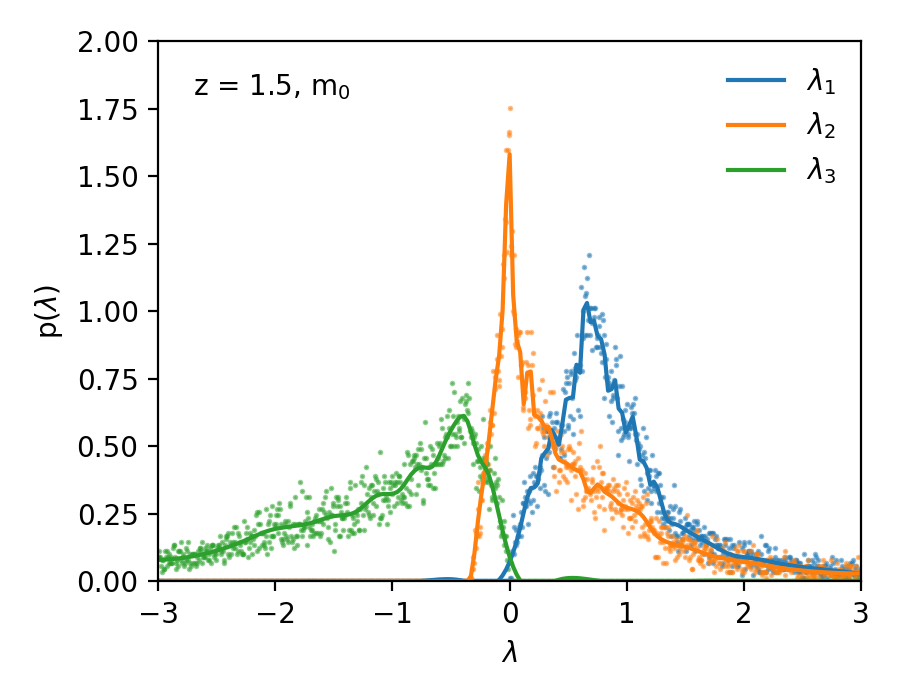
\includegraphics[trim={1cm 0 0 1cm},scale=0.8]{distro_single_light_107.png}
%   \caption{A really Awesome Image}\label{fig:awesome_image2}
\endminipage\hfill
\minipage{0.5\textwidth}%
  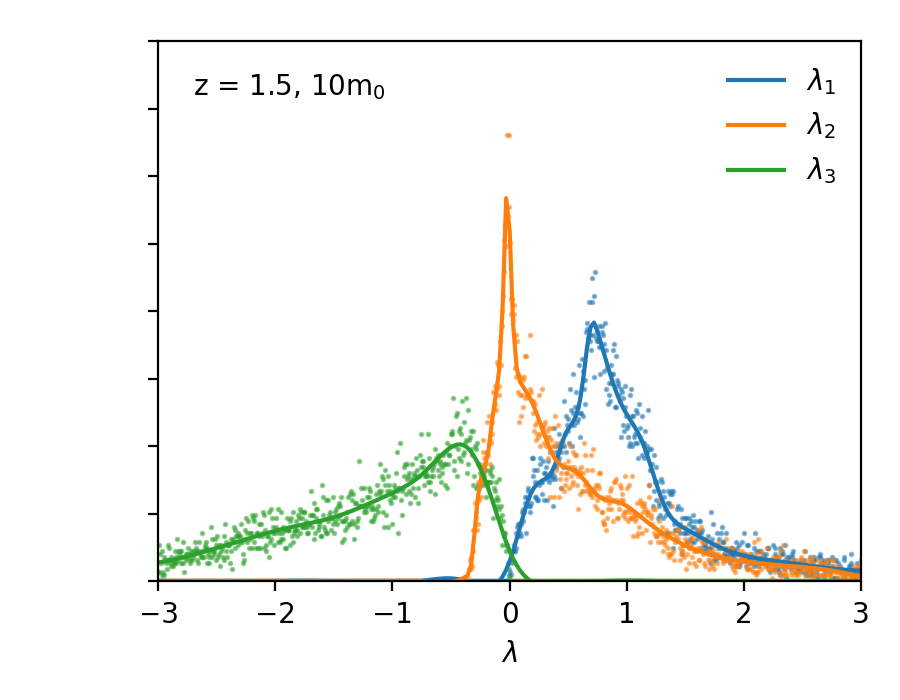
\includegraphics[trim={1cm 0 0 1cm},scale=0.8]{distro_single_mid_107.png}
%   \caption{A really Awesome Image}\label{fig:awesome_image3}
\endminipage
\caption{Singles distros}\label{fig:singles_distros}
\end{figure}



\subsection{Isotropic correlation functions of the eigenvalues of the traceless tidal tensor}\label{sec:iso}

Having demonstrated that the probability distributions of the eigenvalues of the traceless tidal tensor can be used as a measure of the degree of anisotropy in a density distribution, we turn now to the correlation functions of the eigenvalues. We will consider first the isotropic correlation functions in the principal axis frame. 

Before we proceed, it is useful to recall what each eigenvalue represents. To this end, we consider briefly the eigenvalues of the \textit{full} tidal tensor, rather than the \textit{traceless} tidal tensor. Each of these eigenvalues represents the magnitude of the second spatial derivative of the peculiar gravitational potential in one of the three principal axis directions\footnote{It is worth noting that the number of positive eigenvalues of the \textit{full} tidal tensor can, in principal, be used as a classification scheme for cosmological structures. In particular: 0 positive eigenvalues corresponds to a "void", 1 positive eigenvalue corresponds to a "sheet", 2 positive eigenvalues corresponds to a "filament" and 3 positive eigenvalues corresponds to a "cluster". This classification, however, has been shown to be ineffective for inhomogeneous distributions, so we do not consider it here \cite{2016MNRAS.457.2501F}.  
}. The principal axis frame is determined independently for each point of the overdensity field so as to diagonalise the tidal tensor at each point. Each of the eigenvalues can be either negative or positive, representing either convexity or concavity, respectively, of the potential field along the corresponding axis direction. This follows from the usual interpretation of the sign of the second derivative of a curve. We define the eigenvalues such that $\Lambda_1 > \Lambda_2 > \Lambda_3$ (where the capitalisation indicates that these are the eigenvalues of the \textit{full} tidal tensor). Hence, the first principal axis ($\hat{\mathbf{e}}_1$) represents the direction along which concavity is maximal (if $\Lambda_1$ is positive), or convexity is minimal (if $\Lambda_1$ is negative). Conversely, the third principal axis ($\hat{\mathbf{e}}_3$) represents the direction along which convexity is maximal (if $\Lambda_3$ is negative), or concavity is minimal (if $\Lambda_3$ is positive). With this intuition in mind, we return to the eigenvalues of the \textit{traceless} tidal tensor, $\lambda_i = \Lambda_i - \delta/3$. In the traceless case, only $\lambda_2$ may be either positive or negative, while $\lambda_1 > 0$ and $\lambda_3 < 0$. Nevertheless, we still have that $\lambda_1 > \lambda_2 > \lambda_3$, so we can retain the earlier intuition regarding concavity and convexity and use this to predict the behaviour of the correlation functions for different overdensity fields. 

Hence, let us consider an overdensity field in which there are broad troughs in underdense regions but narrow peaks in overdense regions. At a narrow peak (large negative second derivative), we would expect $\vert \lambda_3 \vert$ to be large. Meanwhile, at a broad trough (small positive second derivative), we would expect $\vert \lambda_1 \vert$ to be small. Hence, when looking at the correlation functions of $\lambda_1$ and $\lambda_3$, we would expect the curve for $\lambda_3$ to tend to be higher than that of $\lambda_1$. The opposite would be true for a density distribution with broad peaks and narrow troughs (see Appendix \ref{app:peaks_troughs} for examples). Hence, the relative magnitudes of the correlation functions of these two eigenvalues can inform us about the nature of the underlying density field. Furthermore, we expect density fields which contain clusters to generally exhibit greater $\lambda_1$ and $\lambda_3$ correlations than fields containing extended anisotropic structures such as sheets or filaments (see Appendix \ref{app:peaks_troughs}). We can therefore use this to gauge the relative significance of extended coherent inhomogeneities when comparing different density distributions. 

With these observations in mind, we consider the isotropic correlation functions of the eigenvalues of the traceless tidal tensor for the collapsing overdensities discussed in the previous sections. Again we will compare two cases, m$_0$ and 10m$_0$, at redshifts z = 96.5 (near the onset of collapse) and $z = 1.5$ (relaxed halos). Because of the finite resolution of the simulation grid, the limited number of points to sample at small radii limits the accuracy of the correlation functions at such distances, and thus we plot the correlation functions only for larger radii. Because of this, the impact of small structures present is difficult to determine. Higher resolution simulations in the future should improve these results.  

Figure \ref{fig:iso_corr} displays the isotropic correlation functions of the eigenvalues of the traceless tidal tensor for the collapsing overdensities at redshifts z = 96.5 and z = 1.5. The correlation functions are compared for the ULDM particle mass cases m$_0$ and 10m$_0$. In all cases, it can be seen that $\lambda_1$ and $\lambda_3$ remain coherent over larger scales than $\lambda_2$, for which the correlation function falls off more steeply at large radius. At higher redshift, we see that the correlations are stronger for the higher ULDM particle mass (red lines). This is consistent with the fact that the lower ULDM particle mass case exhibits significant spatially extended interference patterns at this redshift, while these effects are greatly suppressed in the case of the higher particle mass. As discussed above, we expect distributions dominated by cluster-like regions of overdensity to exhibit stronger correlations than distributions dominated by sheet or filament-like structures. Conversely, at low redshift, we see that the $\lambda_1$ and $\lambda_3$ correlations are very similar for both mass regimes. This is indicative of the fact that relaxed halos no longer contain extended sheet-like or filament-like anisotropies, and are instead dominated by incoherent fluctuations. 

Figure \ref{fig:iso_corr} also demonstrates that at both large and small redhsifts, the $\lambda_3$ curve has the highest amplitude at all distances. This is consistent with density distributions containing peaks which are generally broader than troughs, as is expected to arise through gravitational collapse. 

While this analysis is preliminary and does not utilise density distributions from full cosmological structure formation simulations, the differences between the isotropic correlations for the large and small ULDM particle mass cases shown in Figure \ref{fig:iso_corr} indicate that this approach could be utilised to help to constrain the plausible ULDM mass range, or perhaps lend support to either the ULDM or CDM models of dark matter. We note that of course that the anisotropies arise during collapse processes, and are not present in relaxed structures. Therefore this analysis is primarily useful at high redshifts.
 

\begin{figure}[!htb]
\minipage{.5\textwidth}
  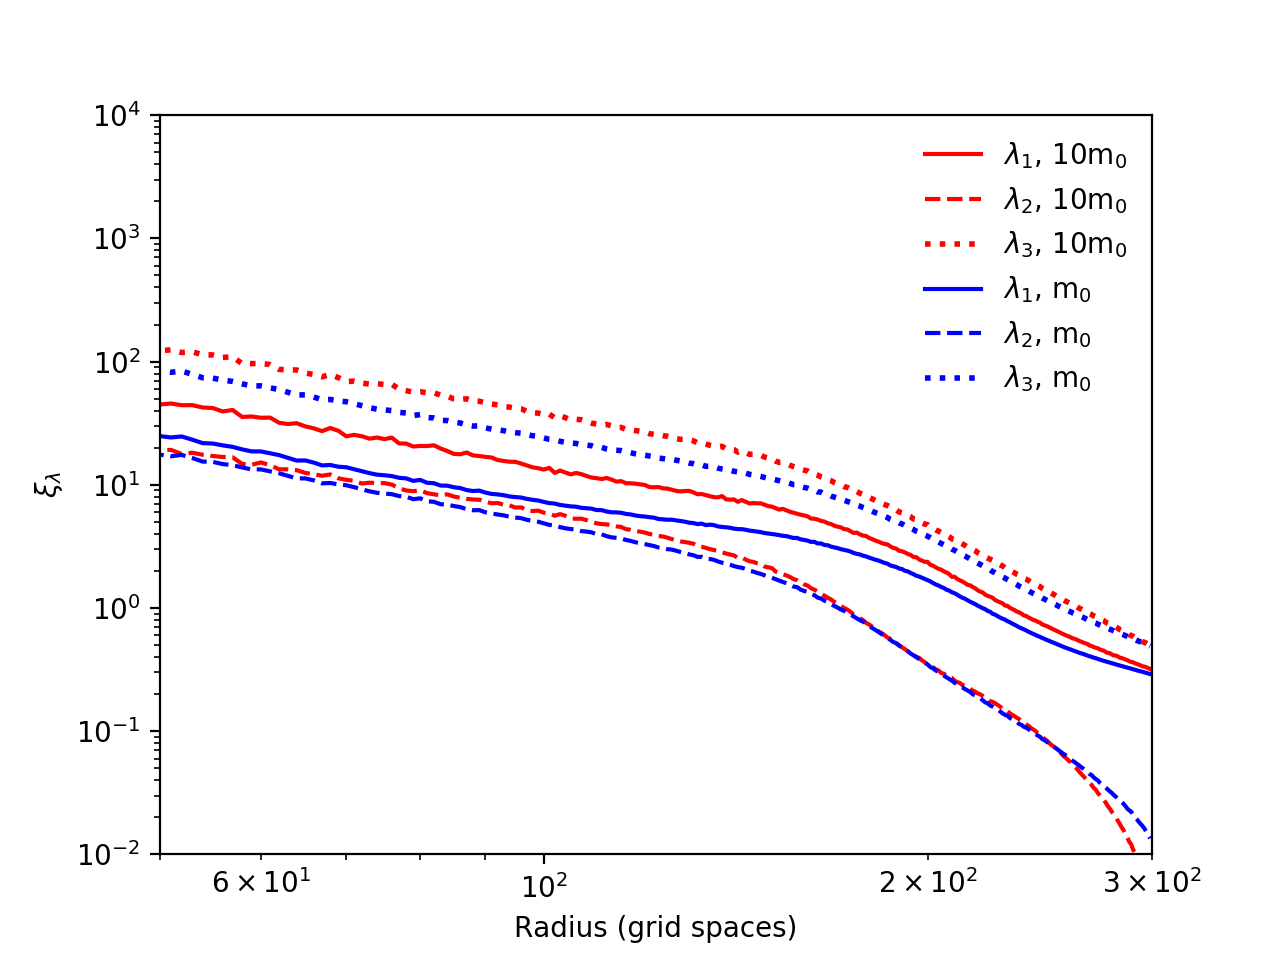
\includegraphics[trim={1cm 0 0 0},scale=0.55]{iso_corr_single_7.png}
%   \caption{A really Awesome Image}\label{fig:awesome_image1}
\endminipage\hfill
\minipage{0.5\textwidth}
  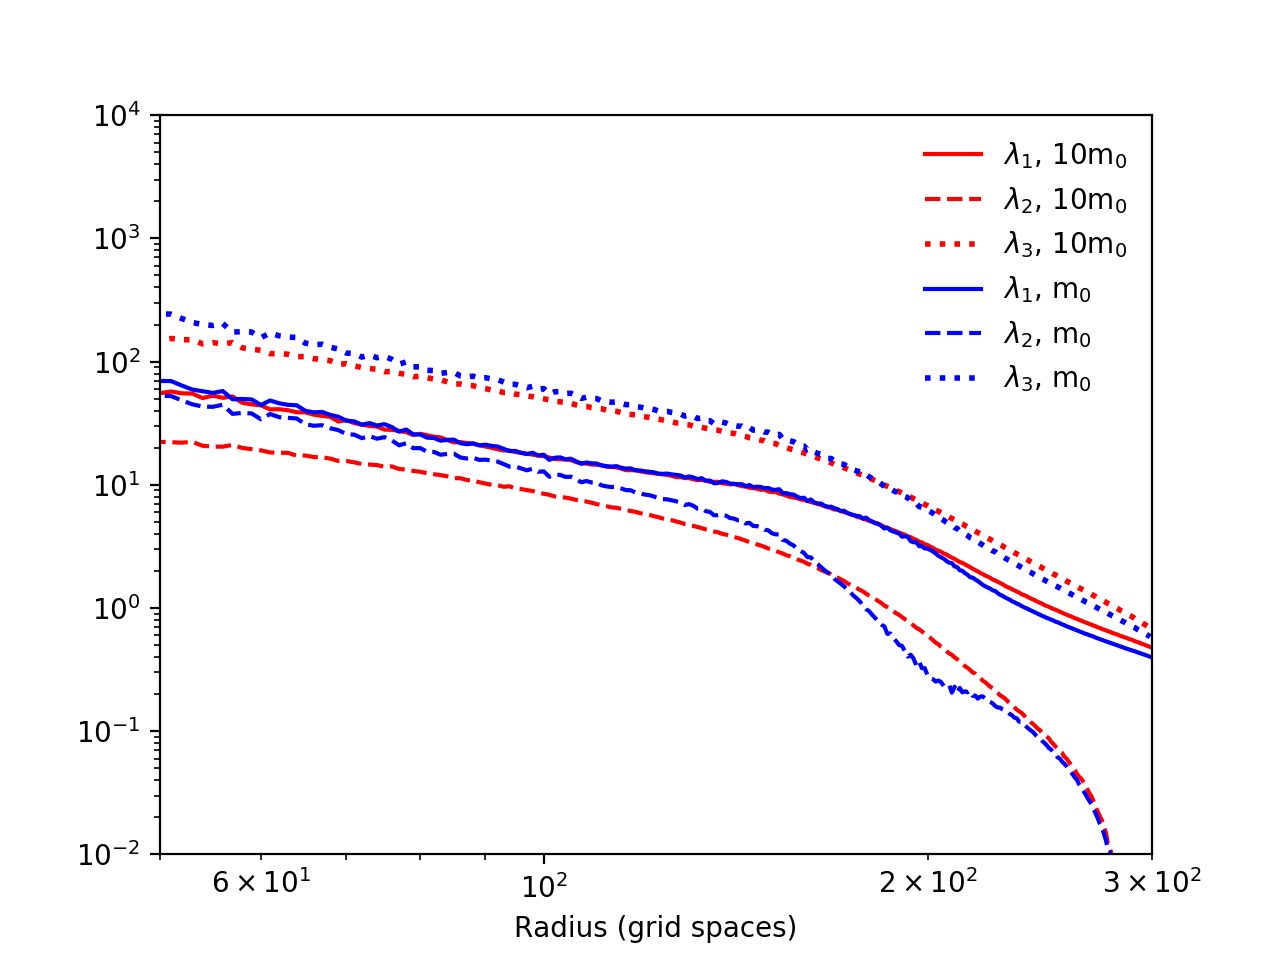
\includegraphics[trim={0 0 0 0},scale=0.55]{iso_corr_single_107.png}
%   \caption{A really Awesome Image}\label{fig:awesome_image2}
\endminipage\hfill
\caption{Isotropic correlation functions of the eigenvalues of the traceless tidal tensor. Left: Correlation functions at z = 96.5. Right: Correlation functions at z = 1.5.}\label{fig:iso_corr}
\end{figure}



%%%%%%%%%%%%%%%%%%%%%%%%%%%%%%%%%%%%%%%%%%%%%%%%


\subsection{Anisotropic correlation functions of the eigenvalues in the principal axis frame}\label{sec:aniso}

In this section we investigate how the correlation functions described above change with angular separation from the $\hat{\mathbf{e}}_1$ principal axis vector. For simplicity, we show only the correlations of $\lambda_1$, as the behaviour of the other eigenvalues is qualitatively similar. 

Figure \ref{fig:aniso} demonstrates the angular dependence of the correlation functions for the largest eigenvalue. We separate the correlation functions based on bins of angular size 15 degrees in $\varphi$ (the polar angle, i.e. anglular separation from $\hat{\mathbf{e}}_1$). We see clearly that the correlations increase with the $\varphi$ in the principal axis frame at all plotted distances. This angular dependence is to be expected, as we expect maximal compression of matter along the direction of $\hat{\mathbf{e}}_1$, resulting in an excess of matter in the plane normal to this vector. As before, the finite resolution of the simulation grid makes obtaining accurate correlations at small distances difficult, so the plots presented here are truncated. 

From this limited data set, it is difficult to extract detailed predictions of the differences between the large and small ULDM mass cases, though it would appear that at early times, angular separation is more pronounced in the lighter mass case. Future investigation of the anisotropic correlation functions characteristic of different ULDM scenarios will benefit from detailed high resolution simulations.



\begin{figure}[!htb]
\minipage{0.5\textwidth}
  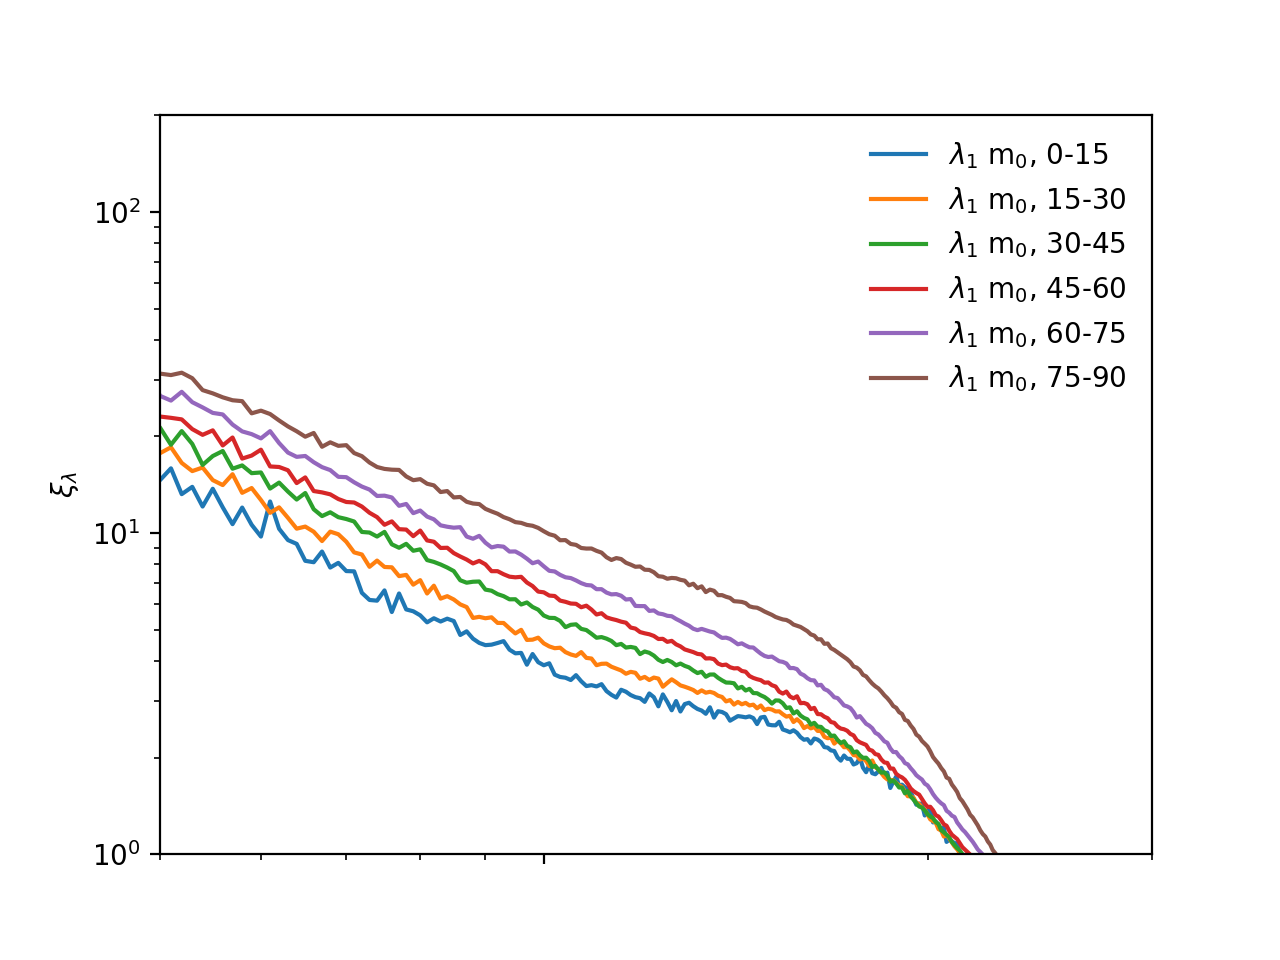
\includegraphics[trim={1cm 0 0 0.5cm}, scale=0.57]{aniso_single_light_7_l1.png}
%   \caption{A really Awesome Image}\label{fig:awesome_image1}
\endminipage\hfill
\minipage{0.5\textwidth}
  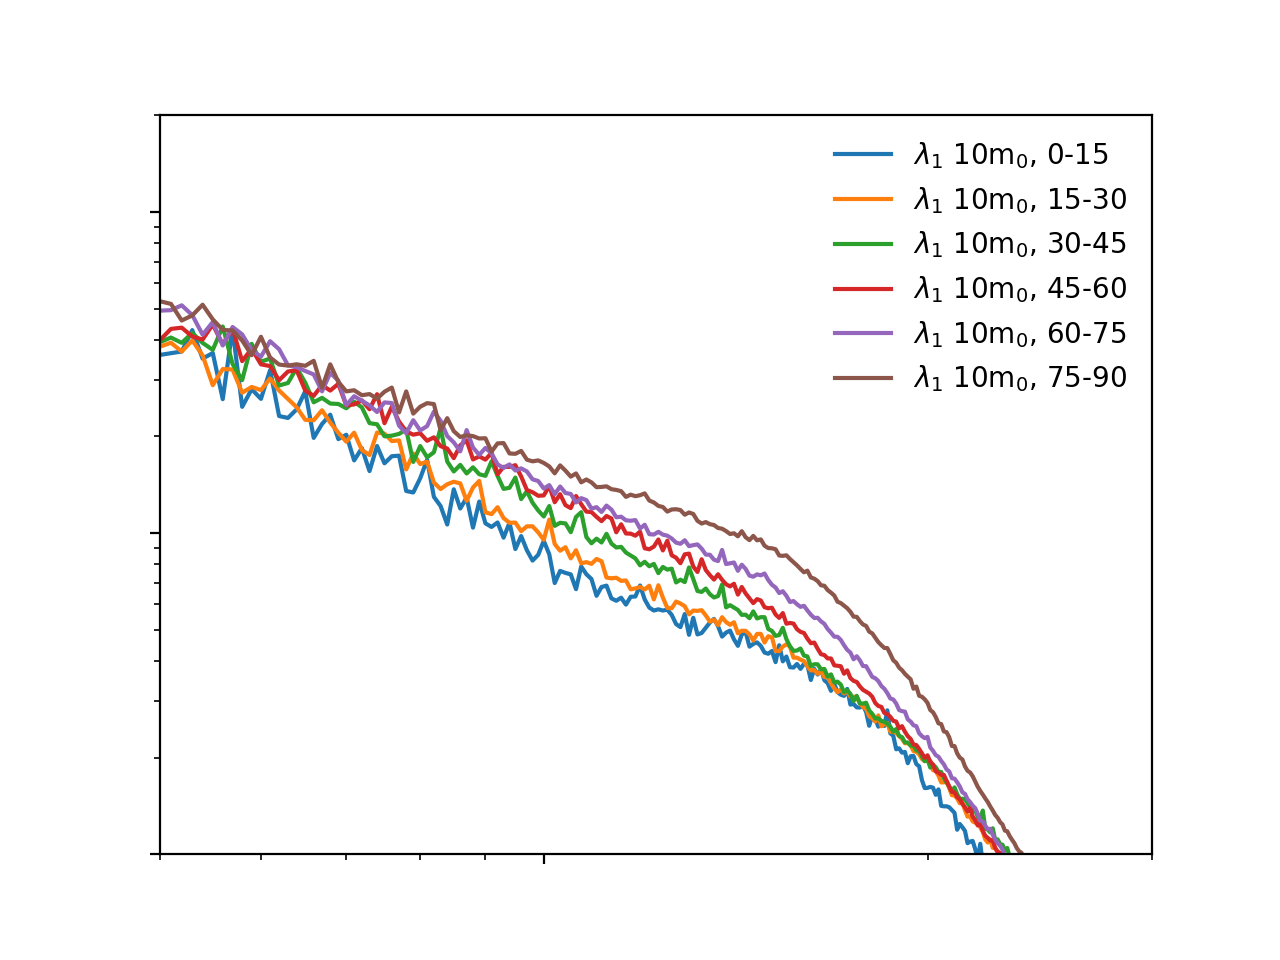
\includegraphics[trim={1cm 0 0 0.5cm},scale=0.57]{aniso_single_mid_7_l1.png}
%   \caption{A really Awesome Image}\label{fig:awesome_image2}
\endminipage\hfill
% \end{figure}

% \begin{figure}
\minipage{0.5\textwidth}%
  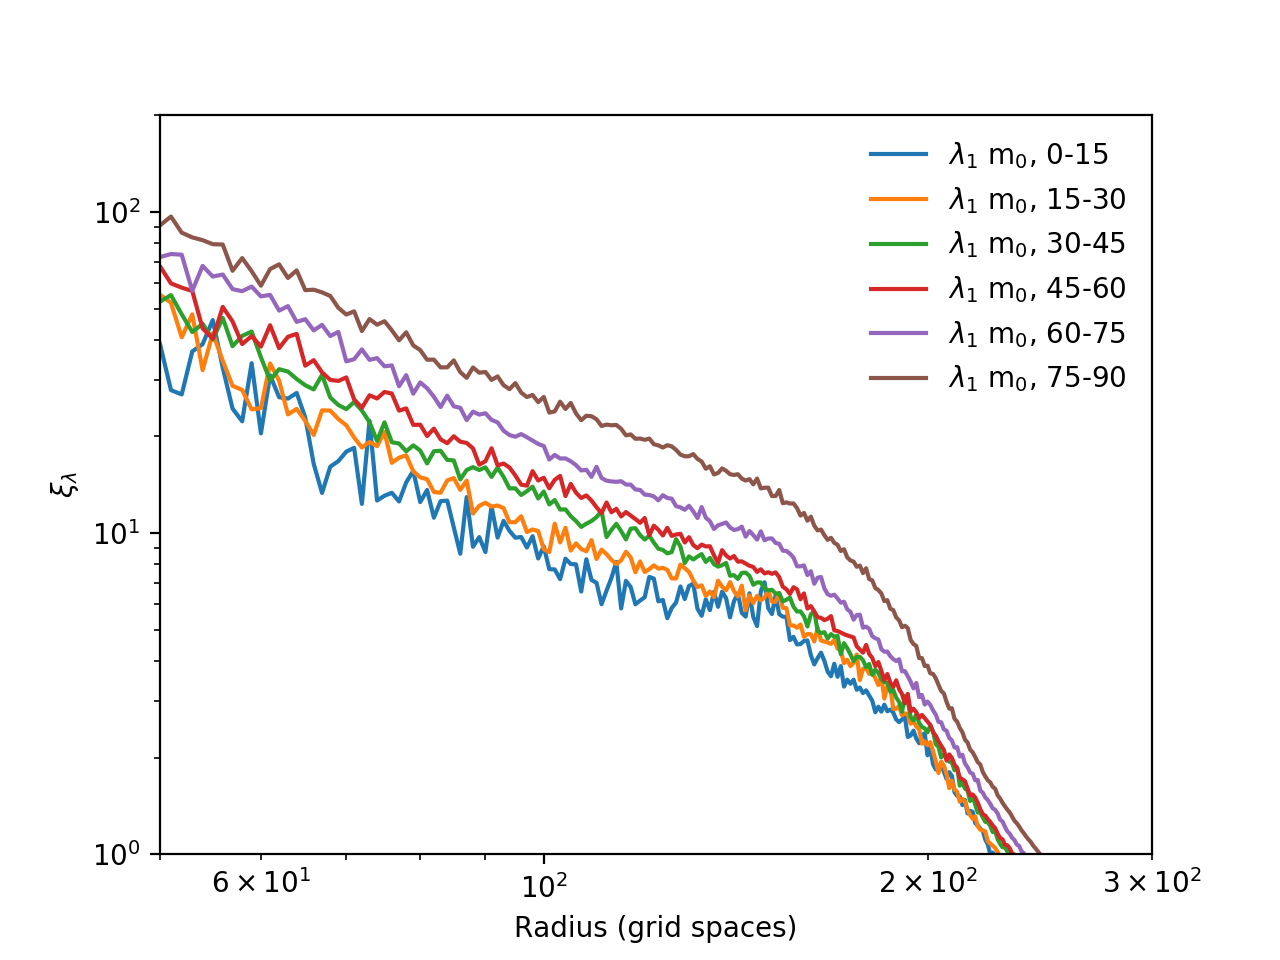
\includegraphics[trim={1cm 0 0 1.cm},scale=0.57]{aniso_single_light_107_l1.png}
%   \caption{A really Awesome Image}\label{fig:awesome_image3}
\endminipage
\minipage{.5\textwidth}
  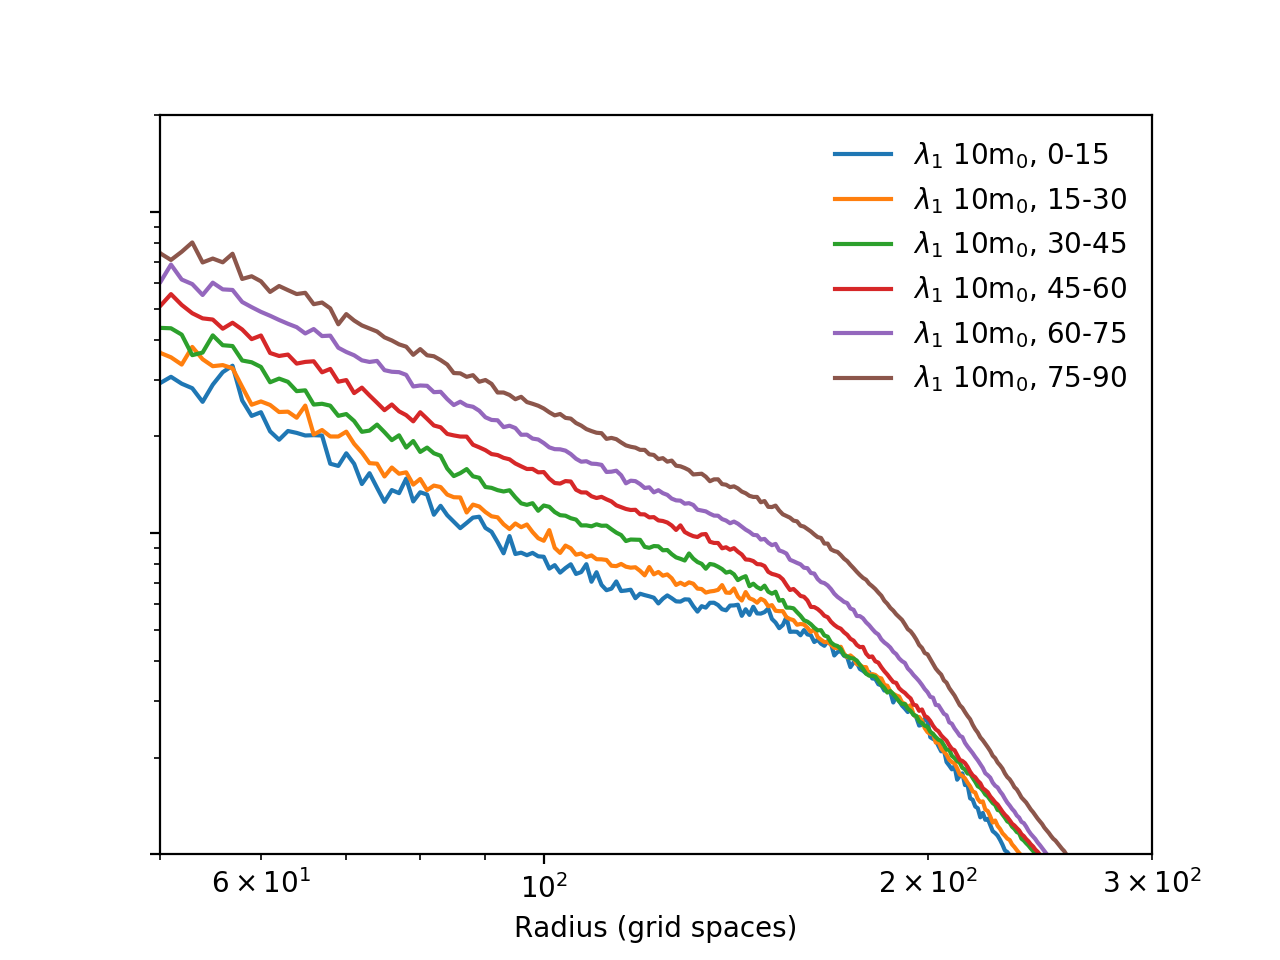
\includegraphics[trim={1cm 0 0 1.cm},scale=0.57]{aniso_single_mid_107_l1.png}
  
\endminipage\hfill
\caption{Anisotropic correlation functions of $\lambda_1$ in the principal axis frame. Top left: z = 96.5, m$_0$. Top right: z = 96.5, 10m$_0$. Bottom left: z = 1.5, m$_0$. Bottom right: z = 1.5, 10m$_0$.}\label{fig:aniso}
\end{figure}



\section{Conclusions}\label{sec:conclusion}

In this paper we have investigated the collapse of isolated ellipsoidal `top-hat' overdensities in the ULDM model. We find that compared to the Zel'dovich collapse of CDM, collapse of ULDM overdensities is greatly influenced by wave effects and interference processes. We see that the gravitational cooling of relaxing ULDM halos is sensitive not only to ULDM mass, but also to the precise shape of the initial overdensity. We also find evidence for rotating solitonic cores in relaxed ULDM halos, though a thorough investigation of this phenomenon requires greater spatial resolution. The ongoing development of AMR codes for ULDM simulations will prove very useful in this regard. We have also presented an example of how variability in the theoretical ULDM core-halo relation can arise. Further investigation into the underlying physics driving this relation is intended for future work. Finally, we also investigated the utility of the traceless tidal tensor as a means by which to characterise the anisotropies in ULDM density distributions arising through wave-like effects on macroscopic scales. We have seen that the probability distributions of the eigenvalues of this tensor exhibit peaks associated with extended filamentary or sheet-like overdensities. The precise position and amplitude of these peaks can be expected to vary with the precise parameters of the underlying ULDM scalar field, and so we suggest that this could serve as a signature through which to determine the suitability of one model over another. Furthermore, we have seen that the correlation functions of the eigenvalues of the traceless tidal tensor can also be used to distinguish between ULDM models with different particle mass parameters. 

Though this work is preliminary in nature, more advanced numerical tools are currently in development which will enable better characterisation of halos and anisotropies within the ULDM model, not just for isolated overdensities, but for large cosmological volumes. The outputs of such detailed simulations can be analysed with the methods employed here in order to obtain a quantitative distinction between different dark matter models. 











\appendix


\section{Distributions of tidal tensor eigenvalues for density field test cases}\label{app:prob_distro_eg}

To illustrate that overdensities containing extended anisotropic structures correspond to eigenvalue distributions possessing characteristic peaks, we consider two artificial distributions. The first distribution is simply a Gaussian random field, while the second is a 2-dimensional plane wavefront, generated by $\rho(x,y,z)=\sin^2{(x)}$. Figure \ref{fig:gaussian_plane_wave} shows the eigenvalue distributions for the two cases. For the Gaussian random field, in which the statistical fluctuations are isotropic, the eigenvalues themselves are characterised by Gaussian distributions. Meanwhile, the 2-dimensional plane wavefront yields eigenvalue distributions with distinct prominent peaks. The exact position and height of the peaks will of course in general depend on the precise parameters of the waveform.


\begin{figure}[!htb]

\minipage{0.5\textwidth}
  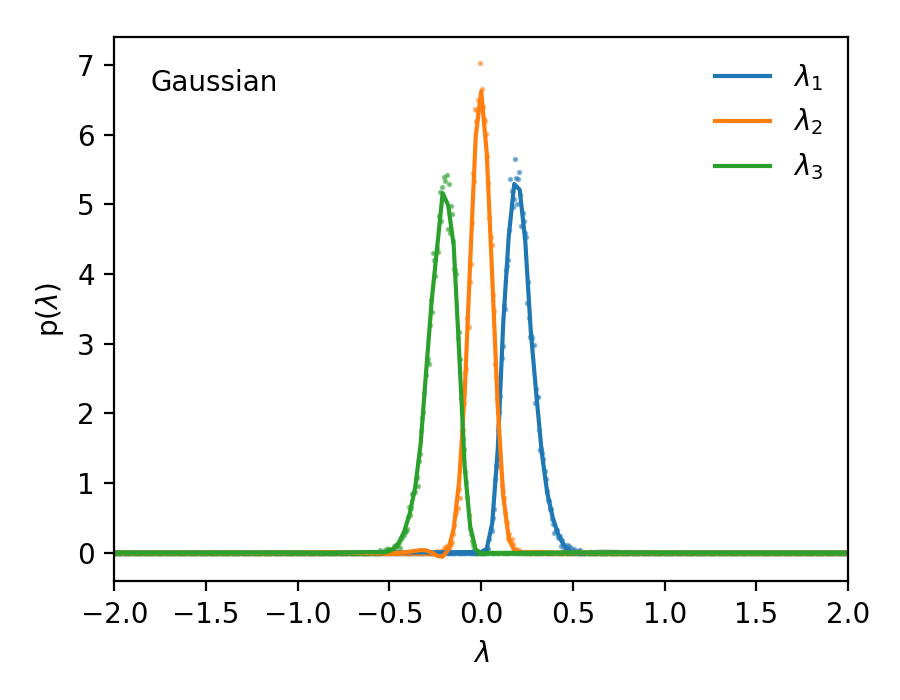
\includegraphics[trim={1cm 0 0 0},scale=0.76]{prob_distro_gaussian.png}
%   \caption{A really Awesome Image}\label{fig:awesome_image2}
\endminipage\hfill
\minipage{0.5\textwidth}%
  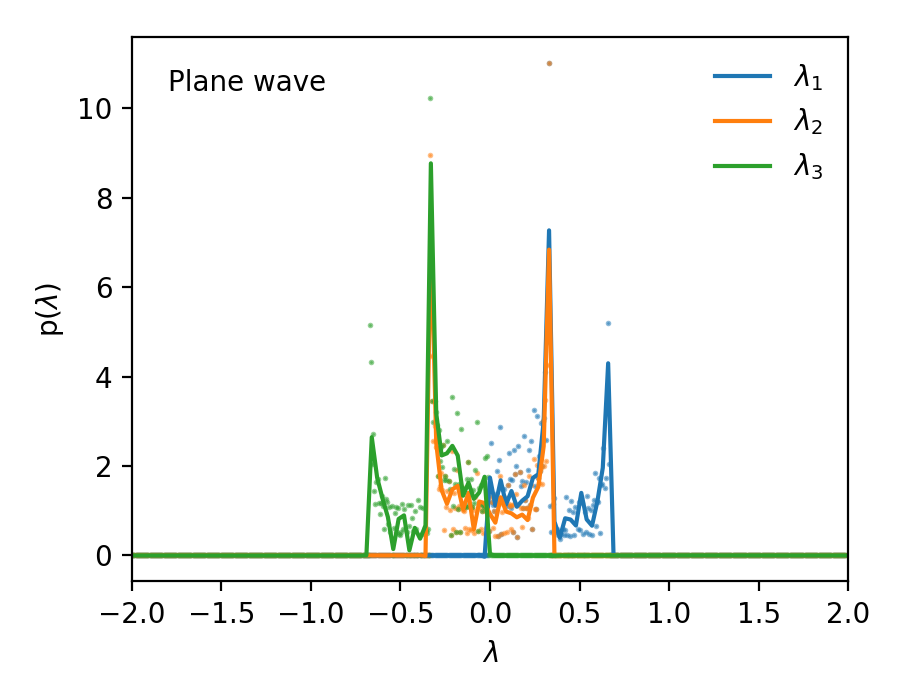
\includegraphics[trim={0cm 0 1cm 0},scale=0.76]{prob_distro_plane_wave.png}

\endminipage
  \caption{Probability distributions of the eigenvalues of the traceless tidal tensor for sample density distributions. Left: Gaussian random field, Right: $\rho(x,y,z) = \sin^2{(x)}$ }\label{fig:gaussian_plane_wave}
\end{figure}


\section{Changes in isotropic correlation functions for sheets, filaments and clusters}\label{app:peaks_troughs}

The relative amplitudes of the isotropic correlations of the largest and smallest eigenvalues of the traceless tidal tensor are dependent upon the characteristic relative sizes of the peaks and troughs of the overdensity distribution. In Figure \ref{fig:iso_comp} we show the correlation functions obtained for artificial density distributions representing sheet-like structures ($\rho(x,y,z) = \sin^2{(x)}$), filament-like structures ($\rho(x,y,z) = \sin^2{(x)}\sin^2{(y)}$), and clusters ($\rho(x,y,z) = \sin^2{(x)}\sin^2{(y)}\sin^2{(z)}$). The method of construction of these structures, namely multiplication of Sine functions, results in asymmetry between the widths of the overdensity peaks and the widths of the underdensity troughs. Because the peaks are relatively sharper, we see that in all cases the amplitude of the correlation function for $\lambda_3$ is higher than that of $\lambda_1$, with the disparity increasing with additional Sine factors.

It is also the case that density distributions dominated by the presence of cluster-like structures will have higher amplitude correlations in $\lambda_1$ and $\lambda_3$ than will distributions dominated by sheets or filaments. This is due to the presence of compression/expansion along additional directions. Hence, Figure \ref{fig:iso_comp} demonstrates that the sheet-like density distribution exhibits the lowest level of correlation, while the clustered distribution exhibits the highest. This increase in correlation with clustering persists even when the precise form of the density distribution is altered, for example exchanging the clustered distribution with $\rho(x,y,z) = \vert \sin{(x)}\sin{(y)}\sin{(z)}\vert$.


\begin{figure}[!htb]
\centering
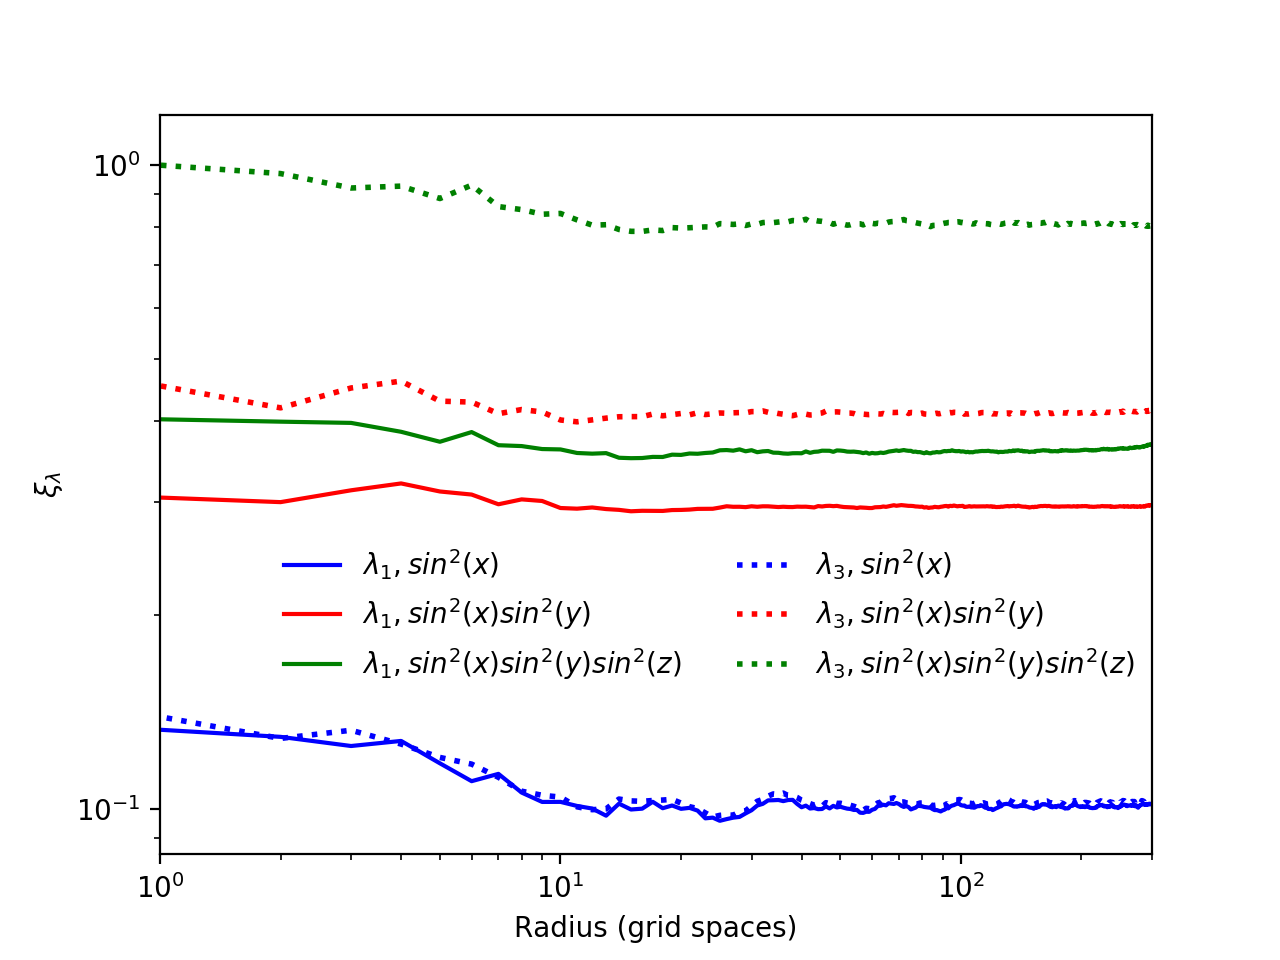
\includegraphics[trim={0 0 0 0},scale=0.8]{sheet_filament_cluster.png}
\caption{Isotropic correlation functions for the largest and smallest eigenvalues of the traceless tidal tensor for different forms of structure (sheets: blue lines, filaments: red lines, clusters: green lines).}\label{fig:iso_comp}
\end{figure}





% \acknowledgments

% \paragraph{Note added.} This is also a good position for notes added
% after the paper has been written.





% The bibliography will probably be heavily edited during typesetting.
% We'll parse it and, using the arxiv number or the journal data, will
% query inspire, trying to verify the data (this will probalby spot
% eventual typos) and retrive the document DOI and eventual errata.
% We however suggest to always provide author, title and journal data:
% in short all the informations that clearly identify a document.

\bibliographystyle{JHEP-mod}
\bibliography{refs} 
\end{document}
